\newtheorem{theorem}{定理}
\newtheorem{definition}{定义}
\newtheorem{lemma}{Lemma}
\chapter{无人机集群自适应协同定位算法}
\section{引言}


微型无人机集群实现高效协同飞行与安全避撞的核心基础在于精确且鲁棒的相对定位。
然而，微型无人机在尺寸、计算资源与通信带宽等方面受到严格约束，使得其在高动态、高密集场景下实现实时相对定位面临显著挑战。
尤其在全球导航卫星系统信号不可靠甚至不可用的环境中，无需外部基础设施、完全依赖机载感知与通信的协同定位技术成为推动无人机集群飞行的关键技术支撑。

尽管现有基于超宽带的集群测距协议能够较为高效地获取无人机之间的距离信息，但这些协议最初并非面向相对定位任务设计，在高密集、高动态集群条件下易受到通信冲突与测距报文不匹配等因素影响导致连续的测距失败，从而极大的制约了定位系统的鲁棒性与可靠性。

针对上述问题，本文首先提出了一种面向相对定位的鲁棒集群ß测距协议。
围绕集群测距中尚未有效解决的核心难题之一，即固定测距周期在高负载条件下易引发持续测距冲突，而随机测距周期又可能导致测距报文不匹配，从而导致无法计算距离。
本文通过理论分析推导出随机测距周期的最优随机化参数，实现了降低连续测距失败现象与报文不匹配之间的有效权衡。
在此基础上，进一步提出了一种权衡测距策略，在测距报文不完全匹配的情况下，利用有限的时间戳信息计算额外的有效距离，从而显著提升测距协议的鲁棒性。

在该测距协议的基础上，针对无人机集群协同定位过程中过程噪声与测量噪声协方差矩阵未知或随时间变化这一固有问题，本文进一步提出了一种自适应扩展卡尔曼滤波方法。
该方法基于在线期望最大化（Expectation–Maximization, EM）算法，对预测误差协方差矩阵和测量噪声协方差矩阵进行联合自适应估计，从而在不依赖精确先验噪声模型的情况下，有效提升定位精度与滤波稳定性。

综上所述，本文提出了一种面向资源受限微型无人机集群的协同相对定位方法，为自主协同飞行提供了稳定可靠的技术基础。


\section{基于超宽带的鲁棒集群测距协议}
\label{sec:Theory}
\subsection{集群测距的现有难题与动机分析}

在先前的研究中，我们提出了一种基于超宽带的集群测距协议\cite{shan2022ultra,shan2021ultra}，该协议能够同时支持无线数据通信与集群测距，使得无人机可以并行获取其与所有对等邻居之间的距离信息。
该协议中仅包含一种报文类型，即测距报文，各无人机按照周期性调度依次发送该报文。
图\ref{fig:3_1}以三个节点的无人机集群为例，展示了该测距协议的基本工作机制。
在该示例中，节点 $A$、$B$ 和 $C$ 轮流发送共六条测距报文。
如图\ref{fig:3_1}(a) 所示,由于无线通信具有广播特性，每一条报文均可被其余两个无人机接收，从而在每次发送过程中产生三个时间戳。
如图 \ref{fig:3_1}(b)所示，由此可见，任意两无人机之间均完成了两轮双向报文交互，最终获得了计算无人机之间飞行时间所需的完整时间戳信息。

\begin{figure}[htbp]
  \centering
  \subfloat[定期广播测距报文\label{fig:3_1a}]{
    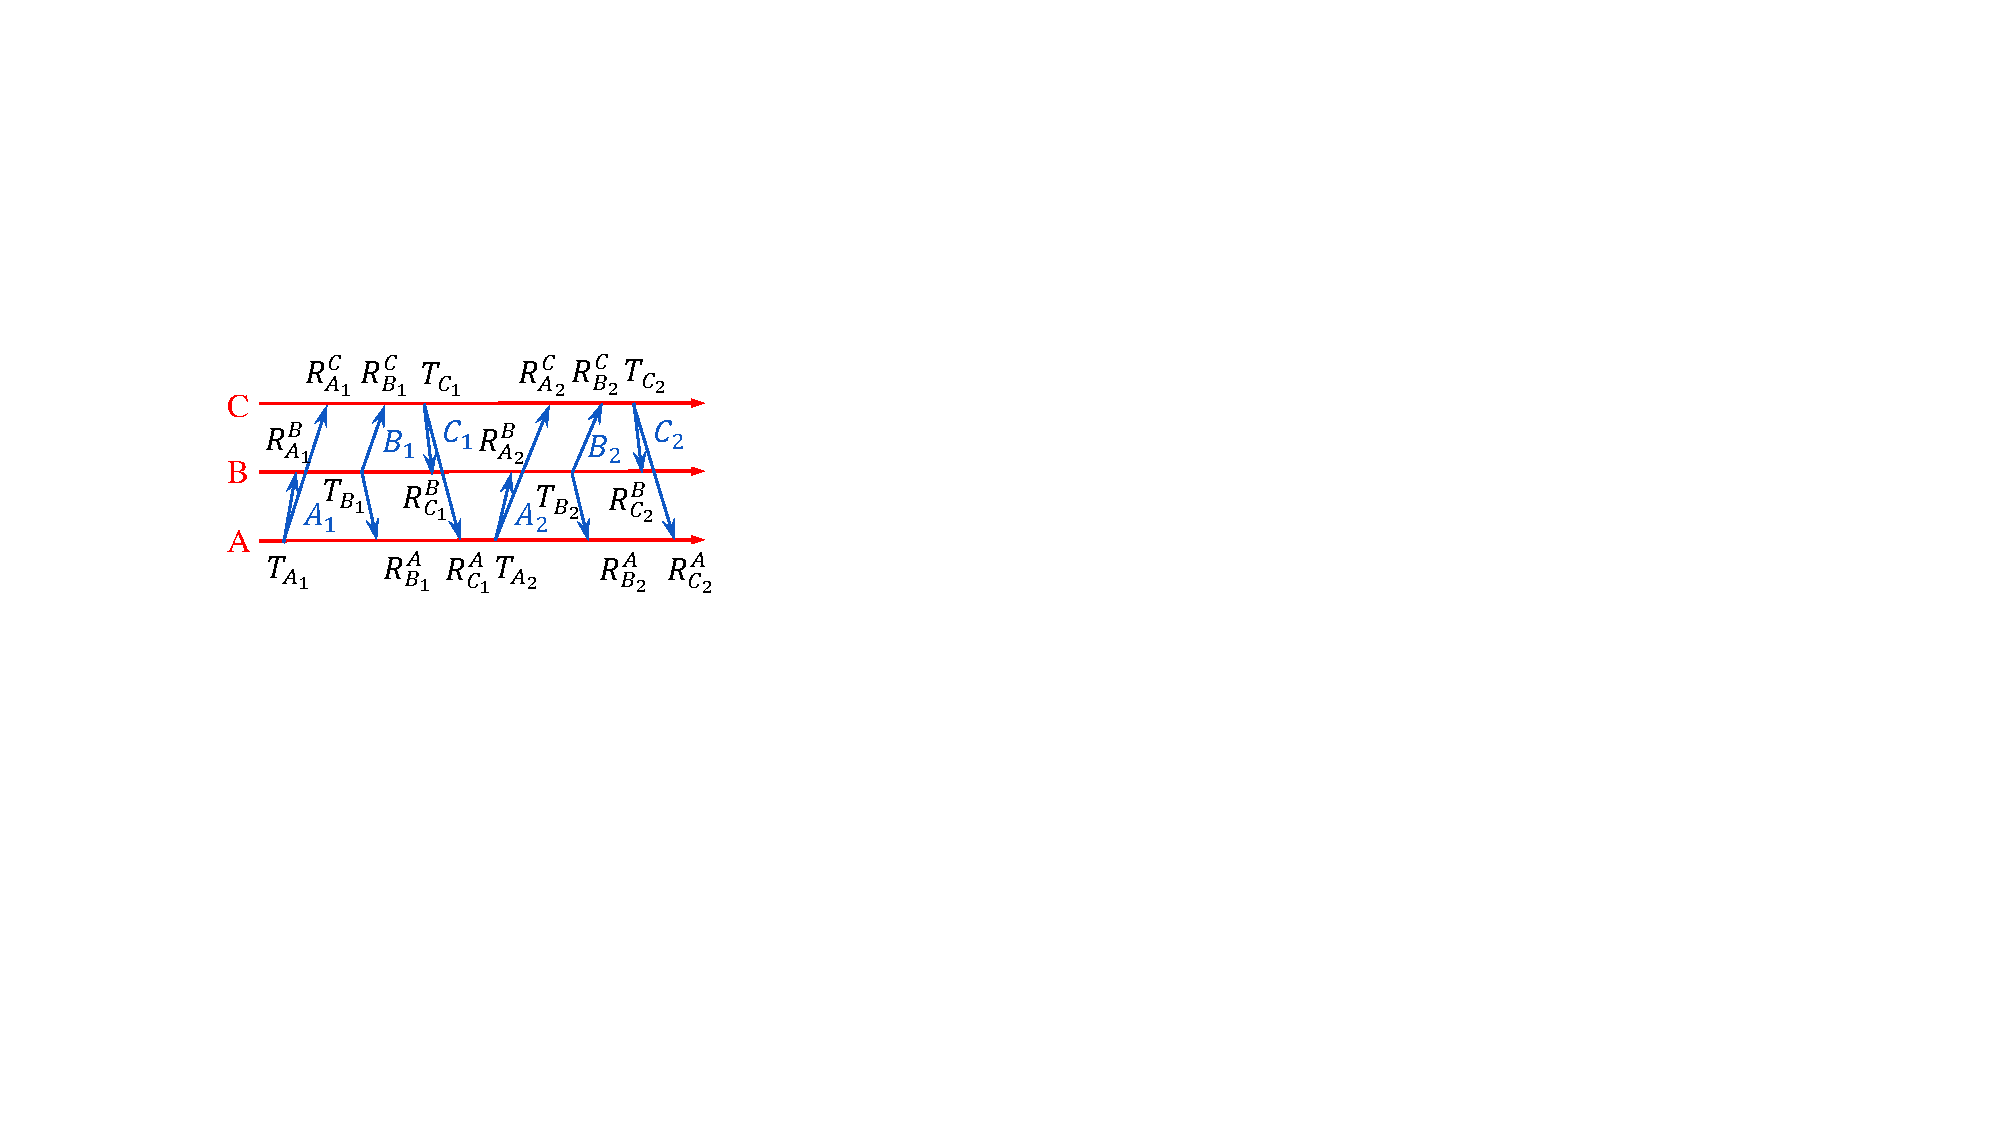
\includegraphics[width=.38\textwidth]{figures/content/chapter3/toyexample1.pdf}
  }
  \quad\quad
  \subfloat[收集足够的时间戳来计算飞行时间\label{fig:3_1b}]{
    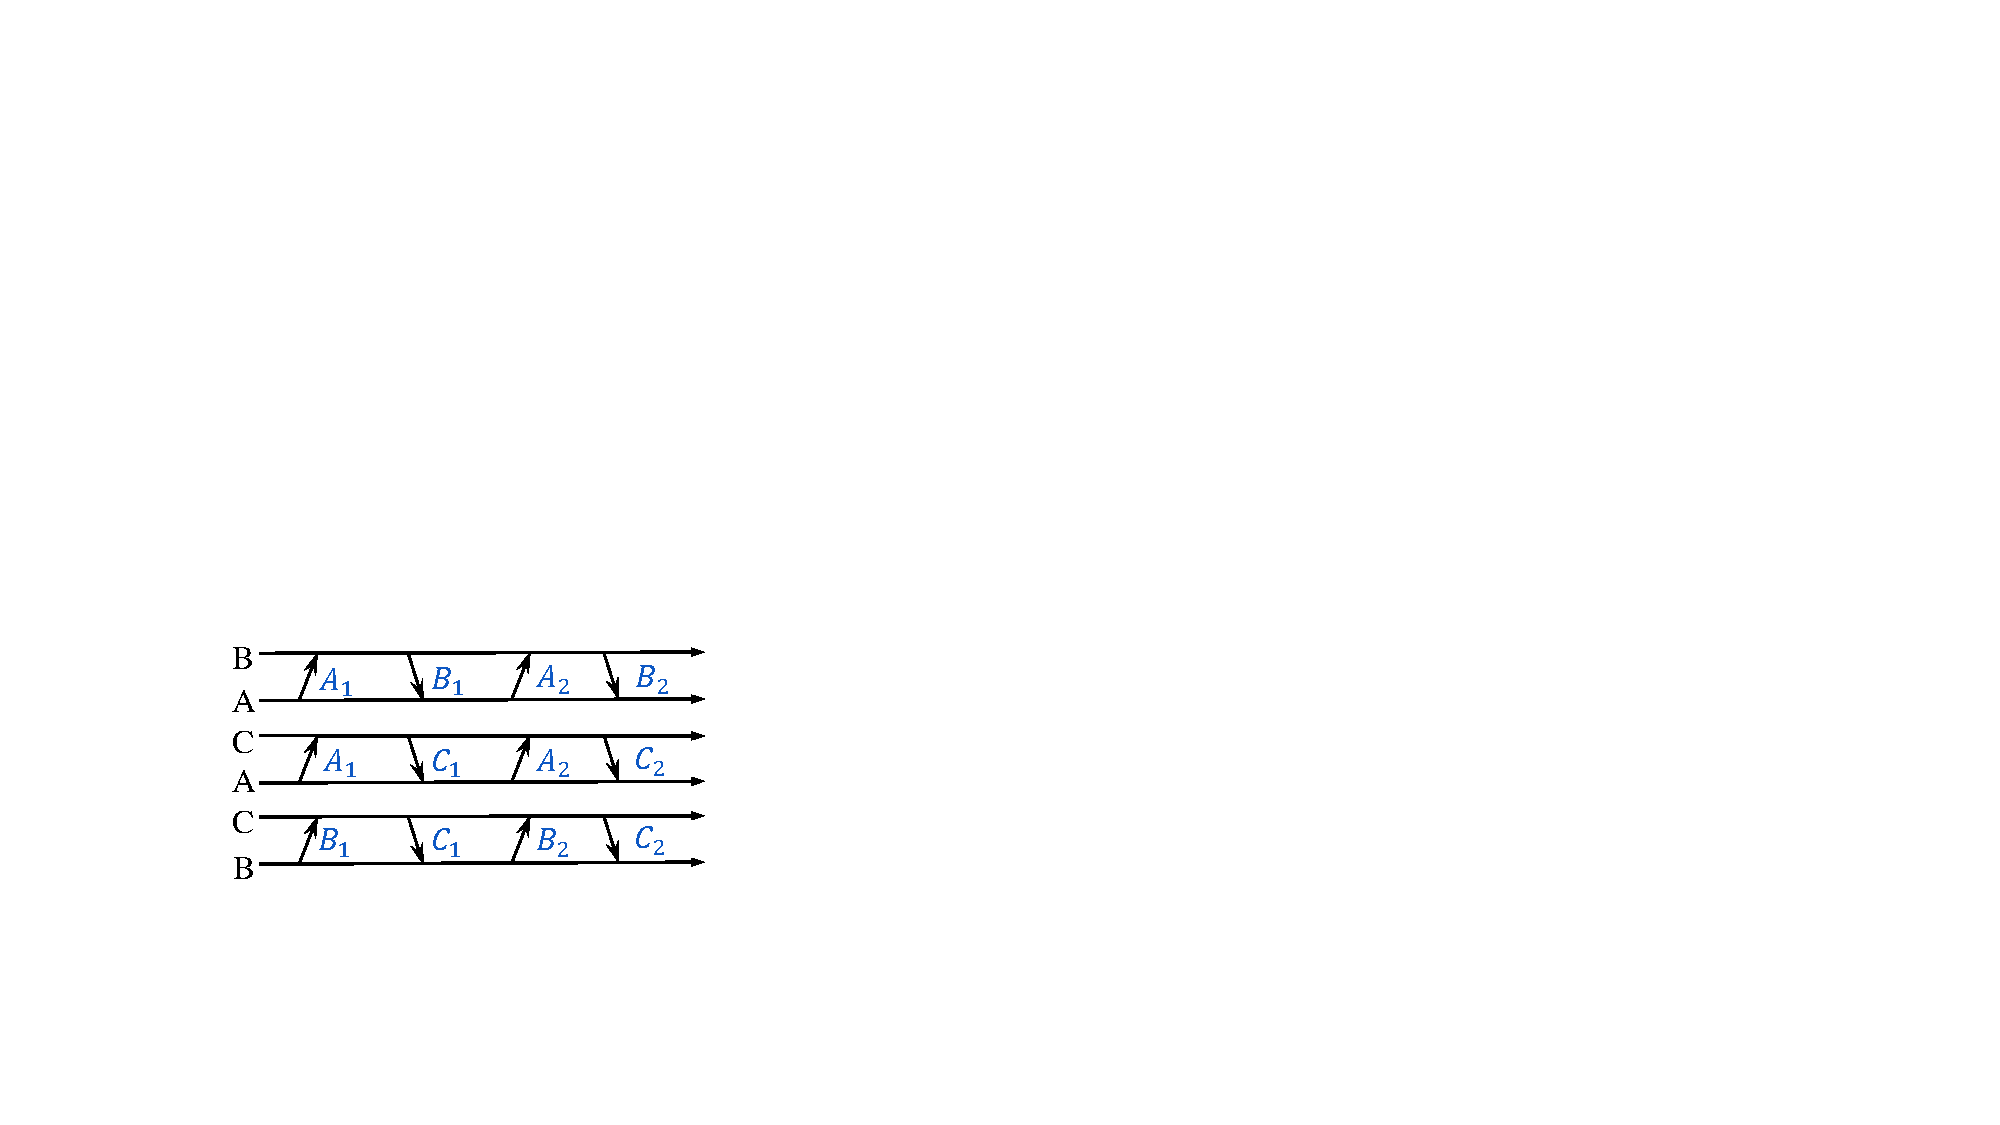
\includegraphics[width=.38\textwidth]{figures/content/chapter3/toyexample2.pdf}
  }
  \caption{无人机集群场景的集群测距协议示意图}
  \label{fig:3_1}
\end{figure}

每个测距报文包含报文标识信息（包括发送无人机的标号及报文序列号）、该无人机最近一次测距报文的发送时间戳，以及从所有邻居无人机节点收集到的接收时间戳。
为了支持相对定位，测距报文必须携带发送方无人机的速度、偏航率和高度信息，以便邻居可以利用这些信息进行相对定位估计。
因此，测距报文的数据字段如图\ref{fig:3_insert}所示。

\begin{figure}[htbp]
  \centering
  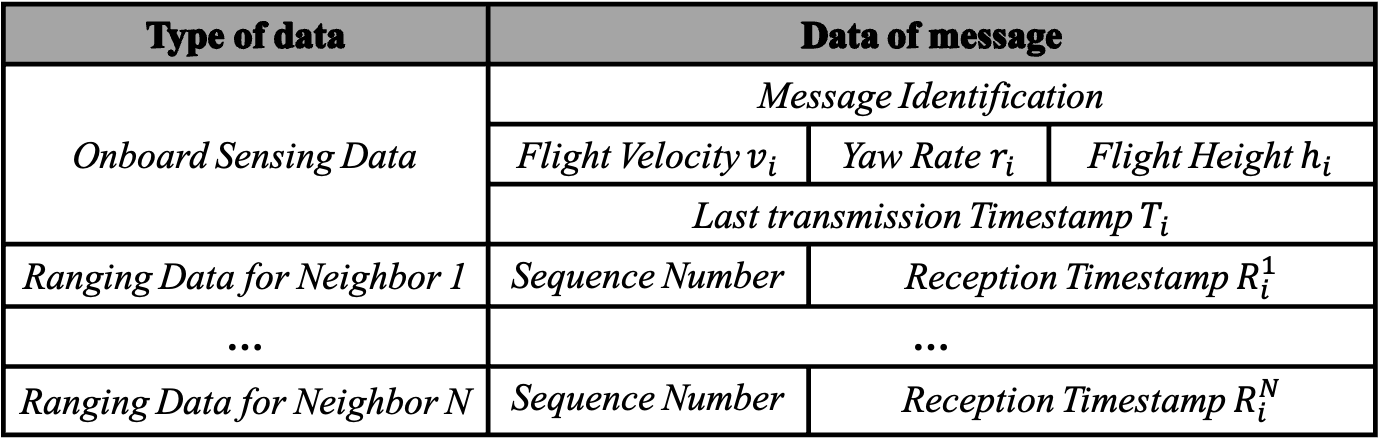
\includegraphics[width=.8\linewidth]{figures/content/chapter3/dataofmessage.png}
  \caption{测距报文中所包含的相对定位相关的数据}
  \label{fig:3_insert}
  \end{figure}


根据飞行时间的计算原理\cite{9179124}，完成一次飞行时间估计需要六个时间戳（$T_p$, $R_p$, $T_r$, $R_r$, $T_f$, $R_f$）。
因此，在该测距协议中，每一个无人机都有一个专用的数据结构，用于存储与其相关的时间戳信息，该数据结构称为测距表。
假设无人机 $A$ 需要与多个邻居无人机进行测距，记$Y$为其中任意一个邻居无人机。
无人机 $A$ 与 $Y$ 之间的报文交互过程如图 \ref{fig:3_2}(a) 所示。
图 \ref{fig:3_2}(b) 展示了无人机 $A$ 在接收到来自无人机 $Y$的第二条测距报文$Y_{2}$时，其测距表中已存储的时间戳信息。
此时，测距表中已包含满足飞行时间计算条件的六个时间戳，从而可以完成无人机$A$ 与无人机 $Y$ 之间的飞行时间估计。

\begin{figure}[htbp]
  \centering
  \subfloat[带有时间戳的报文交换\label{fig:3_2a}]{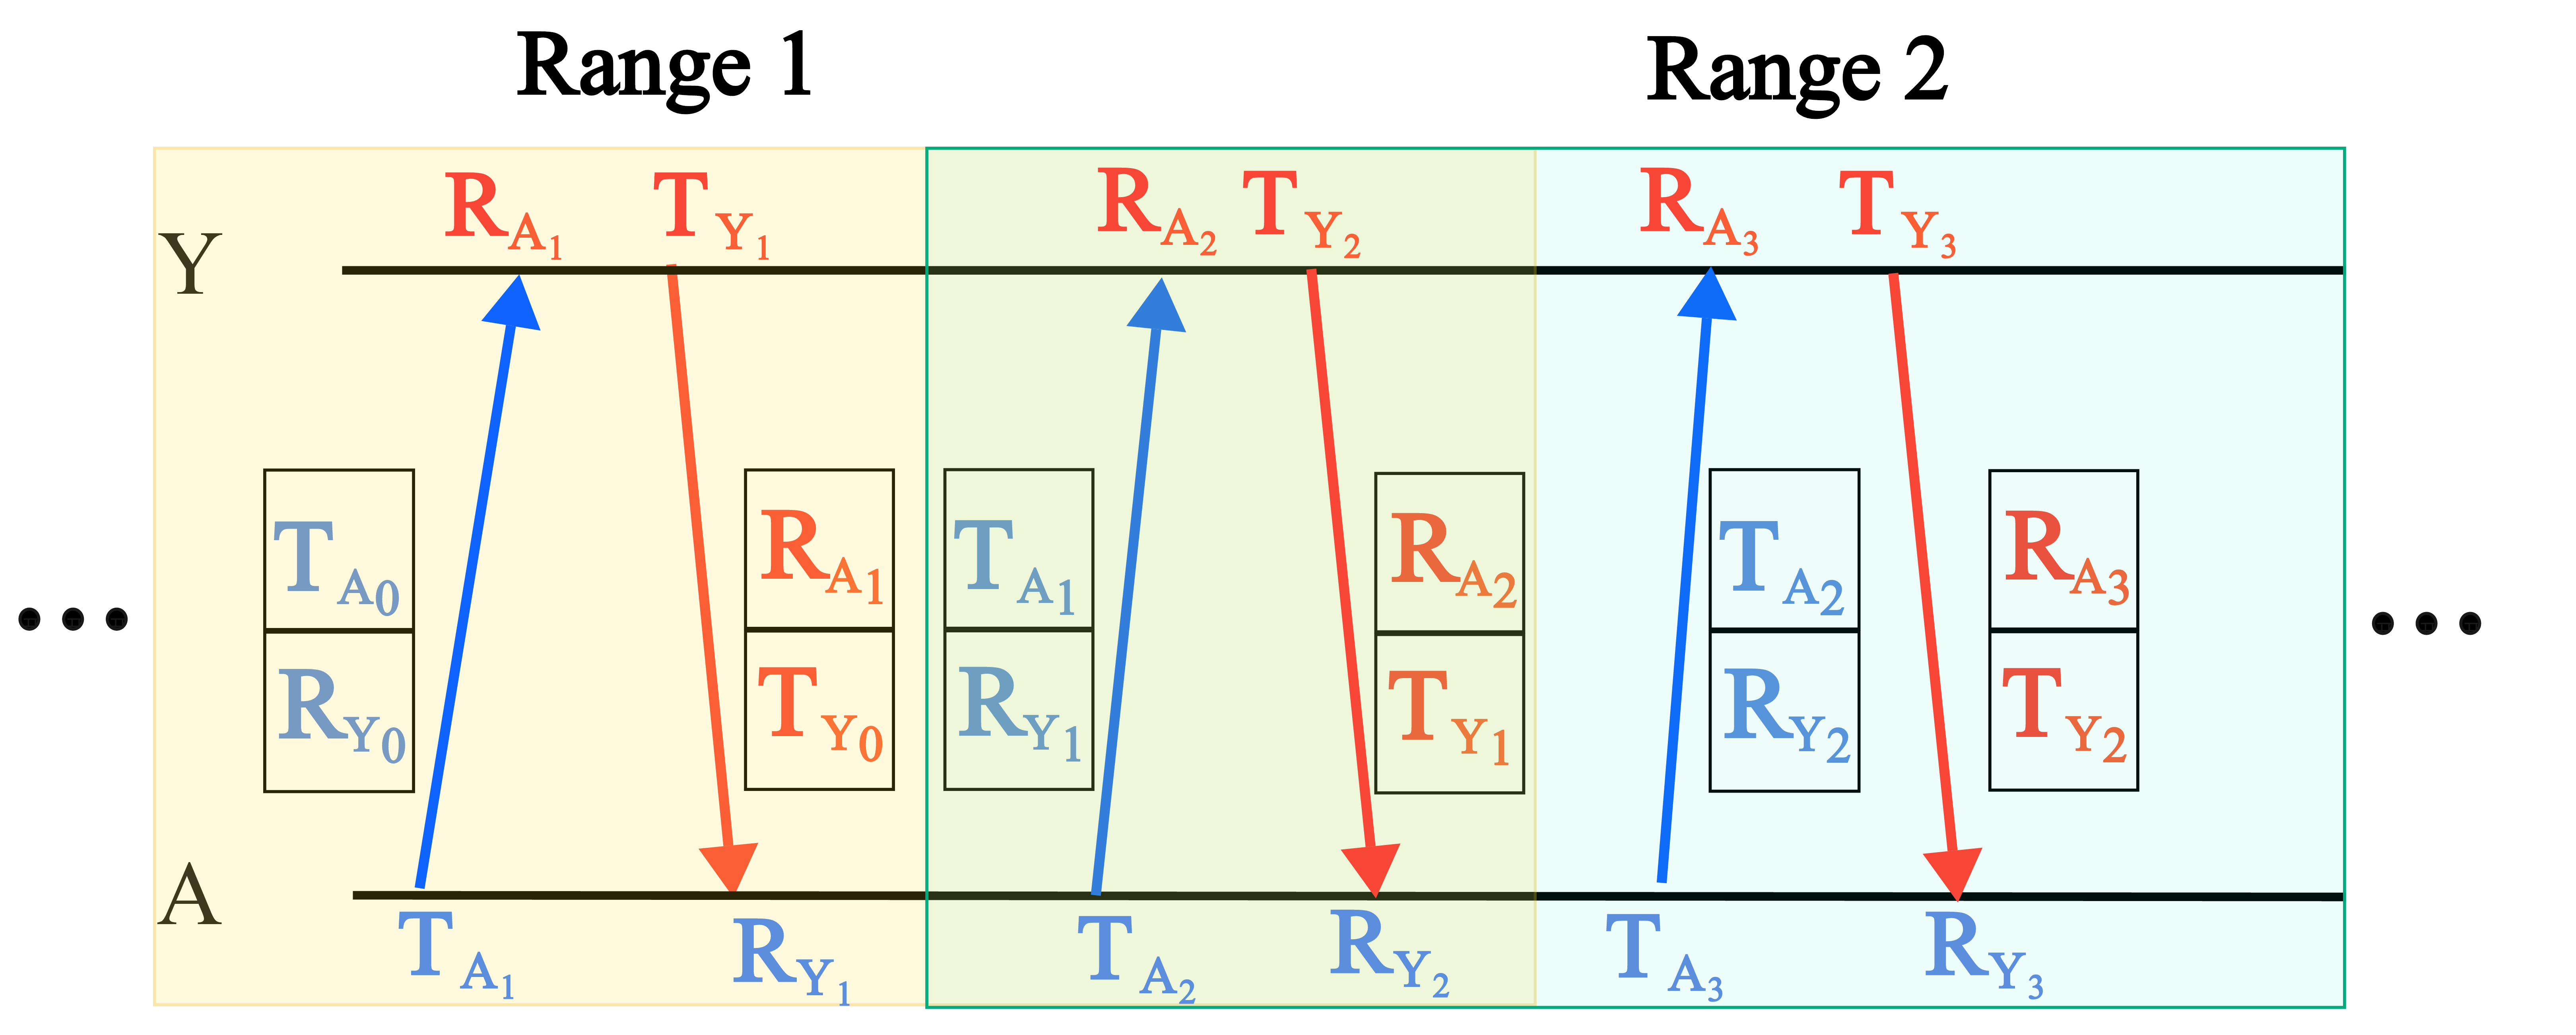
\includegraphics[width=.45\textwidth]{figures/content/chapter3/mes_ex_A_Y.png}}
  \quad\quad
  \subfloat[计算距离的集群测距表\label{fig:3_2b}]{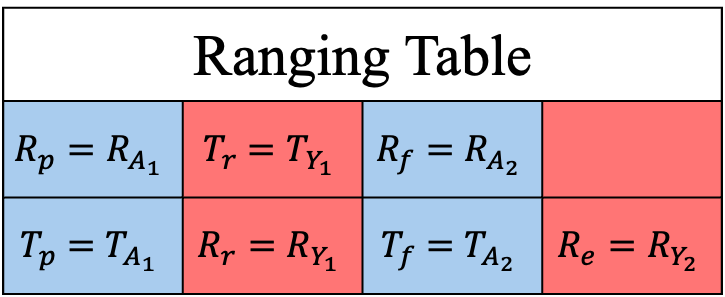
\includegraphics[width=.38\textwidth]{figures/content/chapter3/rangingTable.png}}
  \caption{无人机集群中的报文交换与测距表}
  \label{fig:3_2}
  \end{figure}



在大规模集群测距场景中，众多无人机同时参与集群测距。
各无人机需频繁处理测距报文，包括从邻居无人机接收报文（RX）以及向邻居无人机发送报文（TX），使系统长期处于高通信负载状态。
如图 \ref{fig:3_3} 所示，在理想情况下，无人机报文的发送与接收均按照预设周期进行，两次发送报文时间的间隔具有严格的确定性。
然而在实际应用中，由于硬件芯片普遍存在时钟偏\cite{zhao2022clockids}问题，即使在集群测距协议中为各无人机配置了相同的测距周期，
其本地时钟仍难以实现精确同步，进而导致不同无人机连续两次发送报文的时间戳差值不一致。
如图 \ref{fig:3_4} 所示，不同无人机的时钟存在细微差异，导致 无人机两次发送报文的时间戳随时间逐渐偏移并接近。
最终，两个无人机不可避免地会在非常相近的时间发送报文，从而导致产生长时间的连续测距失败现象。
例如 图\ref{fig:3_4} 中展示的$Y_{2}$，$Y_{3}$报文导致的测距失败。

  \begin{figure}[htbp]
    \centering
    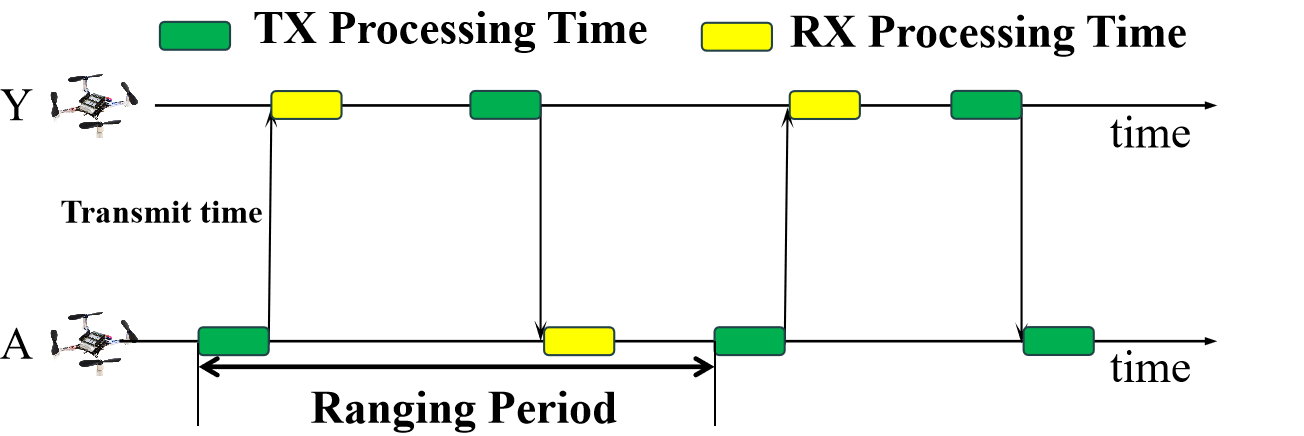
\includegraphics[width=.6\linewidth]{figures/content/chapter3/TxRxProcessTime.png}
    \caption{理想情况下的集群测距}
    \label{fig:3_3}
    \end{figure}

此外，如图 \ref{fig:3_4} 所示，测距报文在网络传输过程中可能发生乱序到达。
例如，来自无人机$Y$的第 7 条测距报文$Y_{7}$可能先于其关联报文到达。
在此情况下，无人机$Y$发送的测距报文无法与无人机$A$发送的关联报文正确匹配，
导致计算飞行时间所需的关键时间戳信息不完整，使得无人机$A$在接收到该报文后无法完成有效测距。
该测距失败的根本原因在于测距报文匹配失败所引起的时间戳缺失问题。
上述问题在无人机密度较高、通信负载较大的大规模集群测距场景中尤为显著，严重制约了系统的测距成功率与整体性能。



\begin{figure}[htbp]
  \centering
  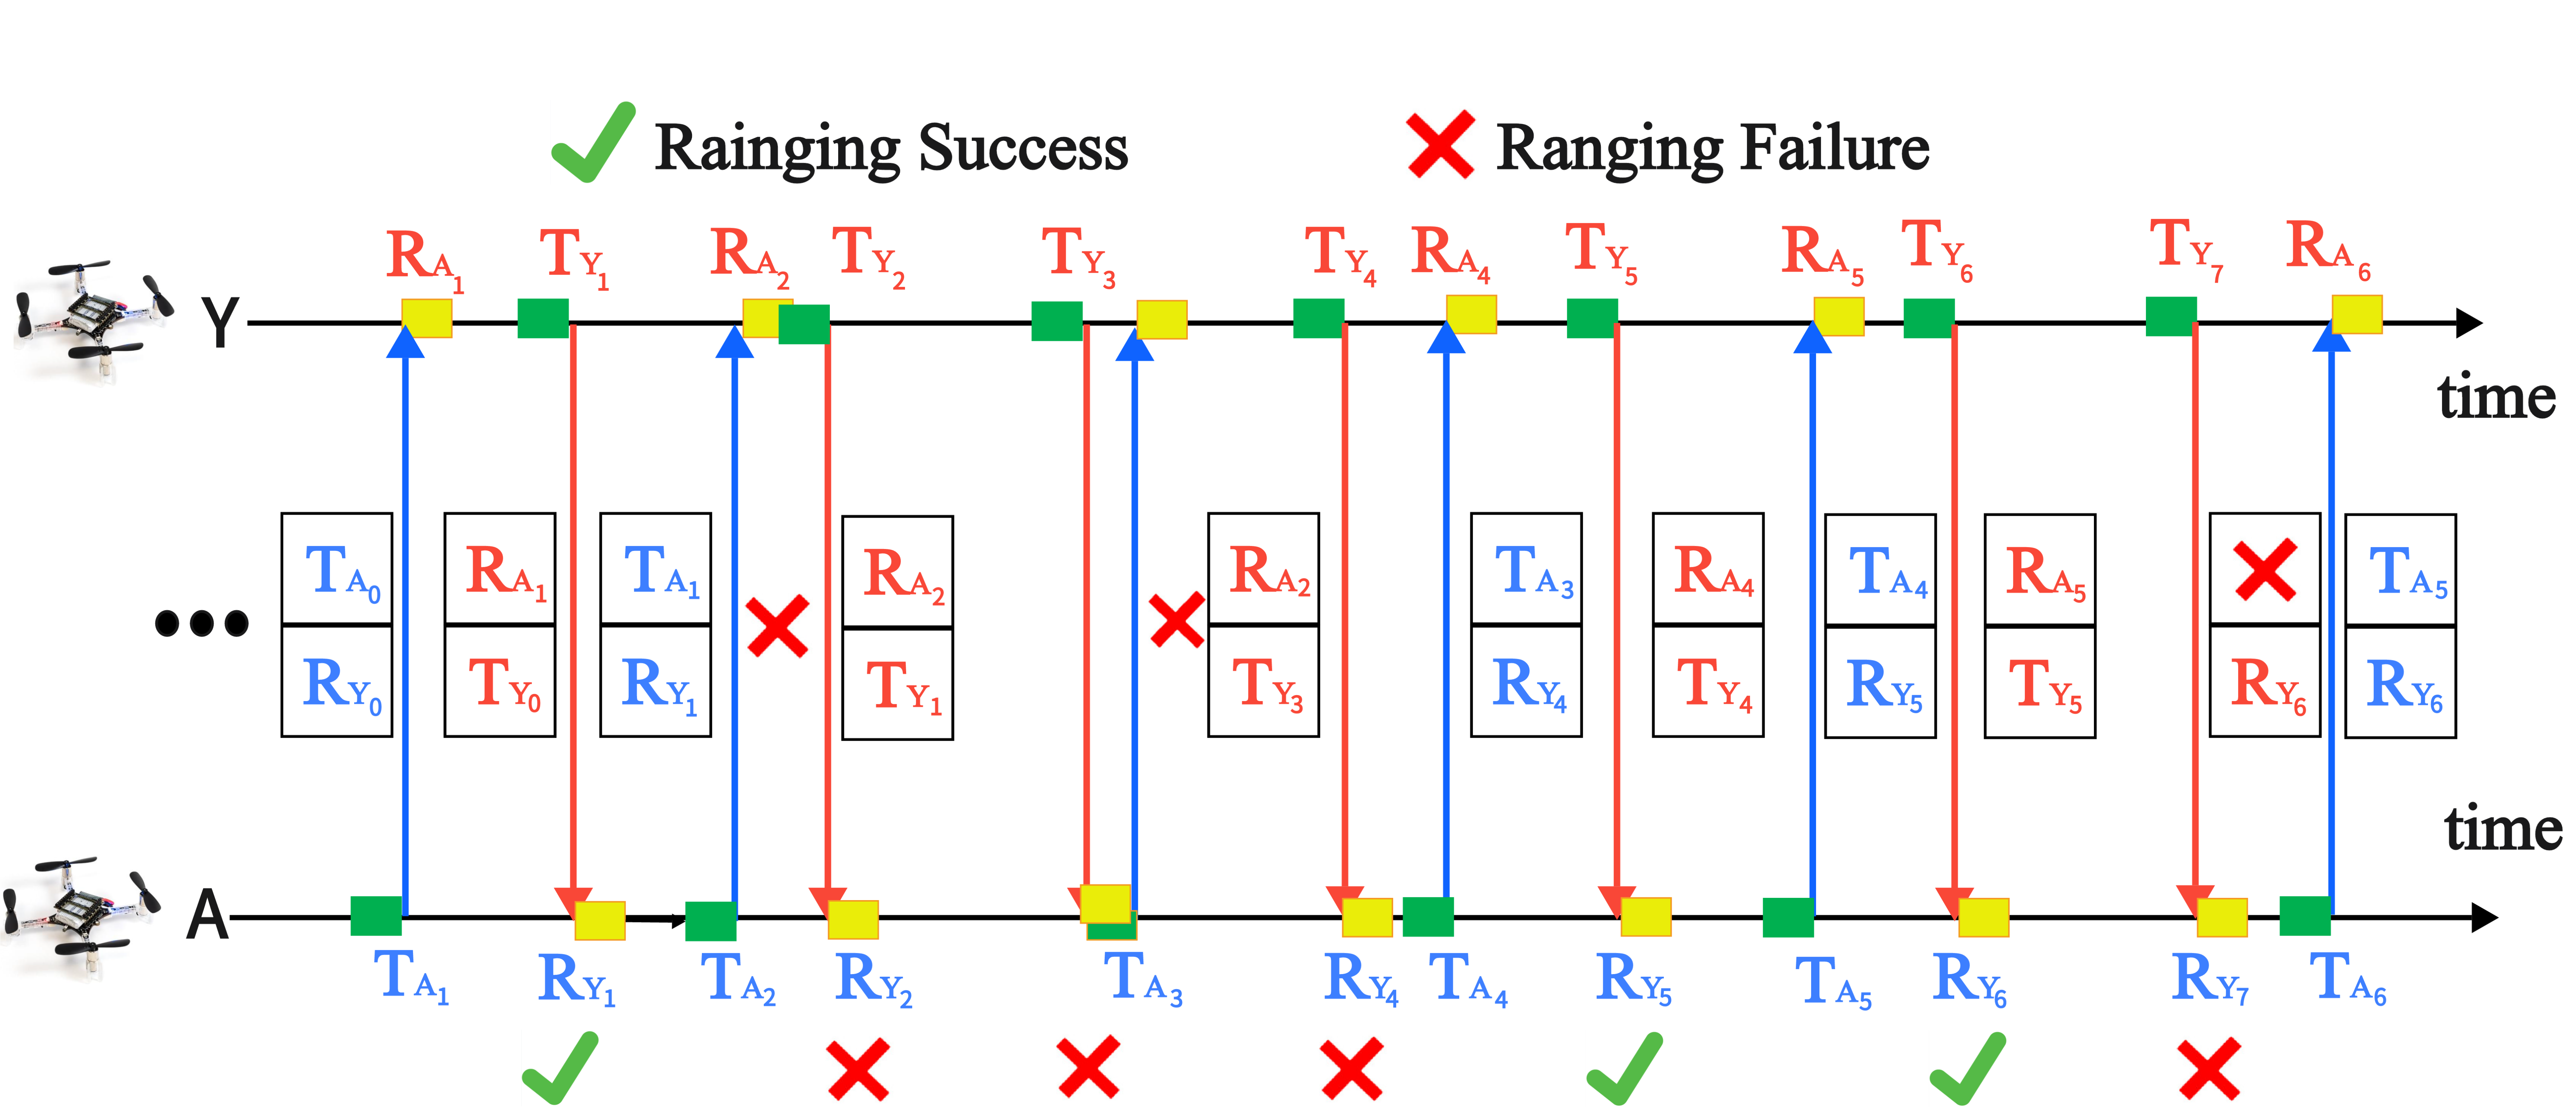
\includegraphics[width=.8\linewidth]{figures/content/chapter3/clockSkew.png}
  \caption{由于时钟偏移所导致的测距失败}
  \label{fig:3_4}
  \end{figure}


因此，我们的研究动机源于三个方面:首先，当我们尝试将此前提出的集群测距协议直接应用于相对定位任务时，会面临着一个难以回避的两难抉择：
一方面，采用静态固定的测距周期，在大规模集群中会不可避免地产生持续的测距报文冲突；
另一方面，引入动态随机的测距周期虽然能够在一定程度上缓解测距冲突，但却会增加测距报文之间无法正确匹配的概率，从而引入新的测距失败问题。
其次，一旦测距报文的交互发生不匹配，部分关键时间戳信息将不可避免地丢失，使得原始集群测距协议无法完成距离计算。
然而，我们注意到，即使时间戳不完整，测距报文中仍可能保留部分有效时间戳信息。
这引出了一个关键问题：在收到报文中存在时间戳缺失的情况下，是否仍可利用现有时间戳信息实现距离估计?
该问题在相对定位应用中尤为关键，也直接促使我们思考设计一种更适用于大规模集群相对定位的新型测距协议。
此外，在通过引入随机性以缓解测距失败时，随机参数的合理选取及其对系统性能的影响仍缺乏系统性的分析与评估方法。
这使得现有测距协议在大规模集群中的性能表现难以预测，也限制了进一步优化的空间。

根据上述内容的分析，测距失败主要由两类原因引起：报文丢失和测距报文不匹配。
对于报文丢失的情况，如图 \ref{fig:3_4} 所示，当无人机 $A$ 在发送自身测距报文时无法接收到无人机 $Y$ 测距报文, 因此无人机$Y$发送的测距报文丢失（如 $Y_{2}$ 和 $Y_{3}$，最终无法计算距离，导致测距失败。

另一方面，在测距报文不匹配的情形下，即便无人机$A$ 成功接收到来自无人机 $Y$ 的测距报文，
该报文中也缺少用于计算飞行时间的关键时间戳（即 无人机$A$报文 的接收时间戳）。
以图 \ref{fig:3_4} 中的报文$Y_{7}$ 为例，由于节点 $Y$ 在发送 $Y_{7}$ 之后才接收到来自 $A$ 的报文 $A_{6}$，导致 $Y_{7}$ 中未包含对应的接收时间戳，从而无法完成飞行时间计算，测距最终失败。

由于硬件时钟偏移通常远小于通信与处理延迟，这类问题往往会导致无人机在一段较长的时间内连续的测距失败。
此外，测距报文混乱交换进一步加剧了报文不匹配现象，显著提高了测距失败的发生概率。

上述分析均已通过实验结果得到验证。
在一组实验中，保持一个无人机静止，另一个无人机以 1 m/s 的速度往返运动，采用原始集群测距协议并将测距周期设置为 $60$ ms。
实验结果如图\ref{fig:3_4} 所示，可以观察到测距过程中周期性地出现连续测距失败的现象，在该实验配置下，每次连续测距失败的持续约 $0.4$ s。

\begin{figure}[htbp]
  \centering
  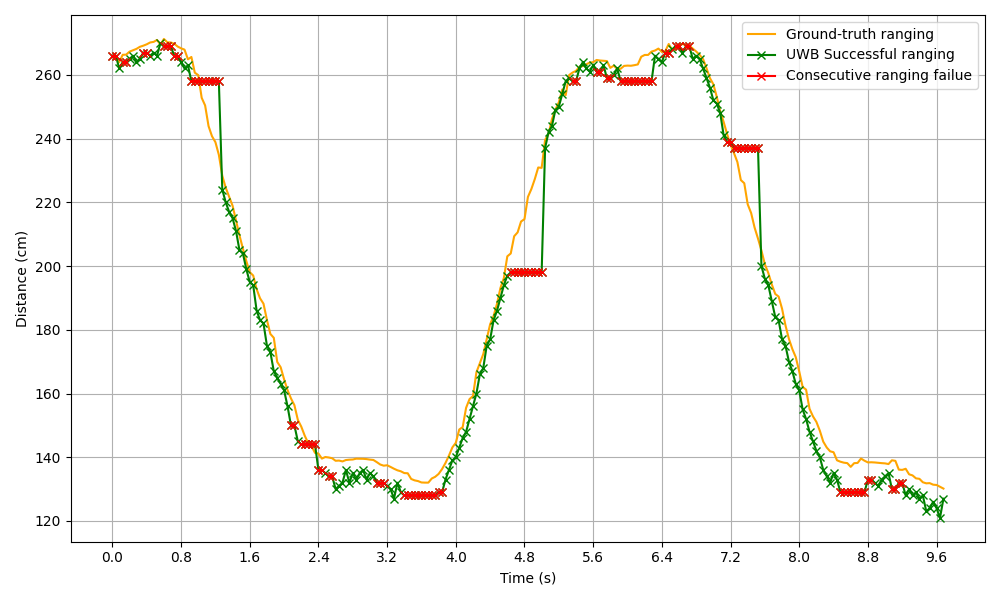
\includegraphics[width=.6\linewidth]{figures/content/chapter3/consecutive_rangingfailuresv2.png}
  \caption{静态的固定测距周期所导致的连续测距失败现象}
  \label{fig:3_5}
  \end{figure}

在另一组实验中，测距周期在 $0–60 $ms 之间随机生成。
实验结果如图 \ref{fig:3_5} 所示，测距失败次数显著增加，从 $9.6$ s 内的 $118$ 次上升至 $9.7$ s 内的 $204$ 次,这些测距失败都是由于测距报文不匹配的原因产生的。

当无人机集群处于高动态、高密集场景时，连续测距失败和测距报文不匹配现象不仅降低了测距可靠性，还会引发额外的通信开销和系统负担。
然而值得注意的是，尽管报文$Y_{7}$ 无法直接用于原始集群测距协议中的距离计算，其仍保留了前一轮测距过程中的发送时间戳。
这一现象进一步启发我们思考：是否可以利用这些残留时间戳信息，实现额外的距离估计？


\begin{figure}[htbp]
  \centering
  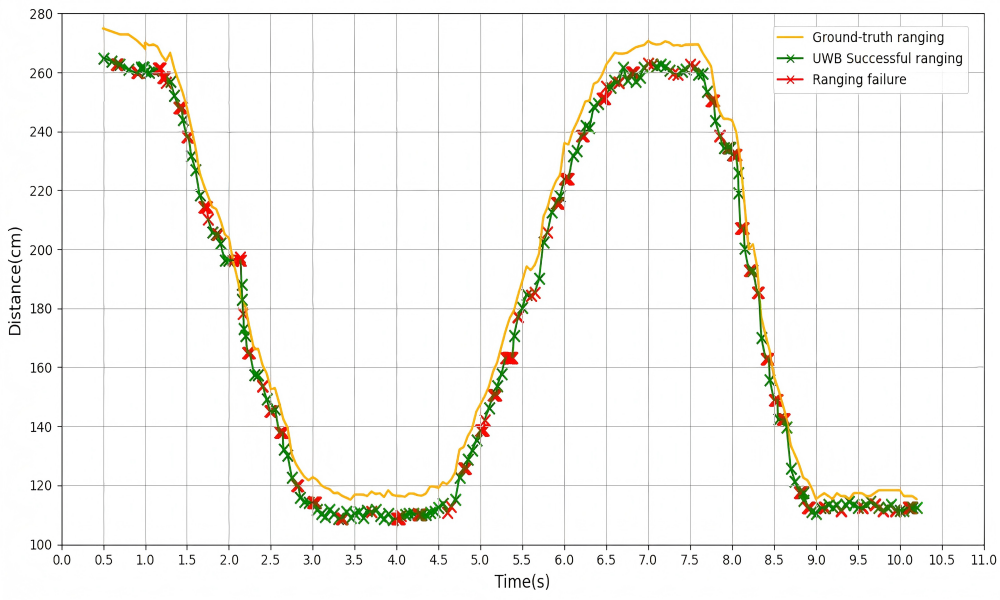
\includegraphics[width=.6\linewidth]{figures/content/chapter3/experiment_w_large.png}
  \caption{测距报文不匹配而导致的测距失败次数增多现象}
  \label{fig:3_6}
  \end{figure}
基于上述分析与实验观察，本文旨在设计一种面向大规模相对定位应用的新型测距协议，以提升在高动态、高密集场景下的测距成功率与系统鲁棒性。
同时，如何系统性地评估该协议在大规模集群中的性能表现，也是本文需要重点关注的问题之一。

下面的小节本文提出并系统分析了一种面向相对定位的鲁棒超宽带测距协议。
该协议首先通过在测距周期中引入随机抖动参数，对测距周期进行随机化，以有效缓解连续测距失败的问题。
然而，抖动的引入也可能带来报文交换不匹配概率增大的风险：当抖动幅度过大时，某一无人机可能在邻居无人机发送下一条测距报文之前连续发送多条报文，
导致这些报文缺乏完整的时间戳信息，使对方无人机无法完成距离计算，最终引发测距失败。
因此，降低报文不匹配发生的概率对于协议的可靠运行至关重要。

针对由报文不匹配导致的时间戳缺失问题，本文进一步提出了一种权衡式测距方法，在鲁棒性与测距成功率之间取得有效平衡。
最后，鲁棒集群测距协议给出了一种高效机制，用于在动态密集集群场景下实现最优性能所需的抖动参数取值，从而提升整体测距稳定性与系统性能。
\subsection{基于扰动的理论分析}
本节首先对由报文冲突导致的连续测距失败次数进行了分析。
直观来看，引入随机化的测距周期似乎可以缓解连续测距失败的问题。
然而，分析结果表明，单纯地增加周期抖动并不能有效降低测距失败的发生频率，因此也无法从根本上减少由报文冲突引起的测距失败。

\begin{definition}[抖动]
测距周期$P$通过引入随机抖动进行随机化处理，其形式为 $P = p + w$。其中，基数 $p$ 为固定值并且$p < P$。
随机变量 $w$ 服从离散均匀分布，其取值范围为 $\left\{0,1,…,W \right\}$，概率质量函数为：
$P(w=k)=\frac{1}{W+1}$。
参数$W$ 被称为随机窗口大小或抖动。因此 ，测距周期的期望值$\overline{P} = E(p + w) = p + W/2$。

\end{definition}

\begin{theorem}
由报文冲突引起的测距失败的平均频率为$\left\lfloor \frac{2L}{\overline{P}^{2}}\right\rfloor$，
其中$L$ 表示 TX 的处理时间。值得注意的是，测距失败的频率与引入的抖动幅度无关。
\end{theorem}

换言之，只要测距周期的期望保持为$P=\overline{P}$ ，是否引入抖动并不会影响由报文冲突导致的测距失败次数。
为证明定理 1，下面首先给出并证明若干引理。

\begin{lemma}
\label{lemma:nojitter}
当不存在抖动（即$W=0$）时，无人机之间可能出现连续的测距失败。
此时，由报文冲突引起的测距失败频率可表示为$f=\left\lfloor \frac{2L}{P^{2}}\right\rfloor$。
    \end{lemma}

证明：考虑两个无人机 $A$和$Y$正在进行集群测距的场景，并且二者采用相同的测距周期 $P$毫秒。
无人机$A$ 和 $Y$ 的单位毫秒时钟偏移率分别记为 $e_A$ ​ 和$e_Y$。
因此，在每个测距周期内，两个无人机累积的时钟偏移分别为 $Pe_A$  ​ 和 $Pe_Y$ 。 
不失一般性，假设 $e_A > e_Y$ ​ 。
则在一个测距周期内，两个无人机之间的报文发送时间差将产生 $P(e_A - e_Y)$ 的漂移。 

当两个无人机之间的报文发送时间差的绝对值小于 $L$  时，其中一个无人机将发生报文冲突并导致报文丢失，从而引发一次测距失败。
由于时钟偏移的存在，这种冲突状态将不可避免地周期性出现。 
我们将连续发生测距失败的时间周期定义为 $P_c=\frac{P}{e_{A}-e_{Y}}$ 。
在一个周期内，测距失败的次数可表示为 $k=\left\lfloor \frac{2L}{P(e_{A}-e_{Y})}\right\rfloor$​ , 而对应的持续时间为 $P_{s}=\frac{2L}{(e_{A}-e_{Y})}$。 
因此，由报文冲突引起的测距失败频率 $ f$ 可计算为$f=\frac{k}{P_{c}}=\left\lfloor \frac{2L}{P^{2}}\right\rfloor$。​\qed

\begin{lemma}
在引入抖动 $W$ 的情况下，由报文冲突引起的测距失败频率仍可表示为$f=\left\lfloor \frac{2L}{\overline{P}^{2}}\right\rfloor$。
  \end{lemma}
证明：
当无人机$A$ 与 $ Y$ 的通信持续时间足够长时，在时钟偏移的影响下，两者的报文发送时间之间必然存在一个时间差 $\Delta t$，其中$\Delta t = TX_{A}-TX_{Y}$。
该时间差  $\Delta t$ 在区间 $[0, P]$ 上服从均匀分布，即 $\Delta t \in U(0, P)$。
 当 $ \left| \Delta t \right | < L $ 时，将发生报文冲突，从而导致测距失败。
 因此，单次测距发生失败的概率为 $\frac{2L}{P}$​ 。 
在引入周期随机化（抖动）后，测距失败的平均发生频率可表示为 $f^{w}=\lfloor \frac{2L}{P^{2}}\rfloor$。
​\qed

由上述分析可知，只要测距周期的期望满足$P=\overline{P}$，则有$f=f^{w}$​，
即无论是否引入抖动，测距失败的总体发生频率保持不变。
这表明，对测距周期设置抖动并不会影响由报文丢失引起的测距失败频率。
换言之，由报文冲突导致的测距失败是不可避免的。

既然由报文冲突引起的测距失败不可避免，那么一个更为关键的问题是：抖动幅度的选择将如何影响 鲁棒集群测距协议在相对定位中的鲁棒性？

以下定理刻画了抖动参数选取过程中所面临的权衡与困境。

\begin{theorem}
连续测距失败平均次数的上确界可计算为 
\begin{equation}
  \sup K_{avg}=1+\frac{2}{W+1}+\frac{1}{W^2+W}, 
\end{equation}
而测距报文不匹配发生的概率可计算为
\begin{equation}
  P(C)=\frac{1}{6P}\frac{W(W^2+3W+2)}{(W+1)^2}.
  \end{equation}
由此可以看出，随着抖动参数 $W$ 的增大，连续测距失败的平均次数虽然有所降低，但测距报文不匹配的概率却随之增加，从而导致整体测距失败次数反而增多。
\end{theorem}

证明：定义事件 $Y_{i}$ ​ 表示发生连续的$i$次测距失败。 
在两个无人机通信测距过程中，精确计算测距失败的概率十分复杂。
为简化分析，本文转而计算连续测距失败平均次数的上确界。
因此，下文给出的概率值均为其上确界。
我们的研究重点在于连续测距失败现象，具体而言，是在发生一次测距失败之后，是否会继续接连不断的发生测距失败。
在该情形下，可以将首次测距失败的发生概率视为 $1$，即 $P(Y_{1})=1$。

当两个无人机进入连续测距失败阶段时，只要它们连续两次发送报文的时间差大于该连续失败阶段的持续时间，则下一次报文丢失将不会发生。
设连续测距失败阶段的持续时间为  $L$ ms。
基于上述分析，在连续测距失败阶段内，两个无人机的测距周期需满足 $\left | P_{A}+P_{A}e_{A}-P_{Y}-P_{Y}e_{Y}\right|>L$,
其中，$P_{A}$ 和$P_{Y}$分别表示无人机$A $和 无人机$Y$ 的测距周期。
在满足上述条件的情况下，将不会发生测距失败。

在实验章节中的实验结果表明，连续测距失败阶段的持续时间满足 $L<1 \text{ms}$。
此外，在单个测距周期内，两个无人机之间的时钟偏移差远小于 $1$ ms。
那么只要下一次测距时引入的抖动满足$w_{A}-w_{Y} \ne 0$，抖动就可以使系统离开连续测距失败阶段。

接下来，我们将分析上述情形发生的概率。
定义 $\Delta w = w_{A}-w_{Y}$, 并记 $\Delta w $ 的概率为 $P(\Delta w)$。
其中， $\Delta w $ 服从表 \ref{tab:Probabilityofdeltaw} 所示的概率分布。

\begin{table}[htbp]
  \centering
  \caption{$\Delta w$ 的概率分布}
  \label{tab:Probabilityofdeltaw}
  \begin{tabular}{|c|c|c|c|c|c|c|c|}
    \hline
    $\Delta w$ 
    & $-W$ 
    & $-W+1$ 
    & $\cdots$ 
    & $0$ 
    & $\cdots$ 
    & $W-1$ 
    & $W$ \\
    \hline
    $P(\Delta w)$ 
    & $\frac{1}{(W+1)^2}$ 
    & $\frac{2}{(W+1)^2}$ 
    & $\cdots$ 
    & $\frac{W+1}{(W+1)^2}$ 
    & $\cdots$ 
    & $\frac{2}{(W+1)^2}$ 
    & $\frac{1}{(W+1)^2}$ \\
    \hline
  \end{tabular}
\end{table}

在无人机进入连续测距失败阶段后，单次继续发生测距失败的概率为 $\frac{1}{W+1}$​ 。
 当$i >1$时， $W$ 取连续  $i$次为 $0$，而第 $i+1$ 次取值不为 $0$，这意味着发生了连续 $i$ 次测距失败。
 因此，连续发生 $i$ 次测距失败的概率  $P(B_{i})$ 可表示为 $\frac{W}{(W+1)^{i}}$。
 由此，可以计算连续测距失败次数平均值的上极限为：

\begin{equation}
\begin{aligned}
\sup K_{avg}&= \lim_{i \to \infty} \sup E(k)=\sum_{i=1}^{\infty} iP(Y_{i})\\
&=1+2\frac{W}{(W+1)^2}+3\frac{W}{(W+1)^3}+...+i\frac{W}{(W+1)^{i}}\\
&=1+\frac{2}{W+1}+\frac{1}{W^2+W}\\
\end{aligned}
\end{equation}

在对测距周期进行随机化之后，连续测距失败的概率将随着 $W$ 的增大而逐渐降低。
与此同时，连续测距失败问题也将得到显著缓解。

接下来，为了尽量减少测距报文不匹配的发生，我们对测距报文不匹配的概率进行分析。
我们考虑在足够长时间的通信测距过程的条件下，计算两个无人机发生测距报文不匹配的概率。
定义事件 $C$ 为两无人机之间发生了一次测距报文不匹配。
显然，当 $W$ 取值过大时，事件 $ C$ 的发生概率将显著升高，这不是我们所期望的。
因此，需要对 $ W$ 的取值范围加以限制，以尽可能降低事件 $C$ 的发生概率。
如图 \ref{fig:3_7}展示了一种特殊情形。
在该情形下，无人机 $A$ 发送了一次测距报文，而无人机 $Y$ 恰好发送了两次测距报文。
其中，无人机 $Y$ 的测距周期在连续两次中均取最小值 $P-\frac{W}{2}$ ，而无人机 $A$ 的测距周期取最大值 $P+\frac{W}{2}$。
只要$W$ 的取值范围满足 $2(P-\frac{W}{2})>P+\frac{W}{2}$, 即 $W<\frac{2P}{3}$​ ,
即可保证在两个无人机同时发送测距报文之后，事件 $ C$ 不可能会发生。 
 \begin{figure}[htbp]
  \centering
  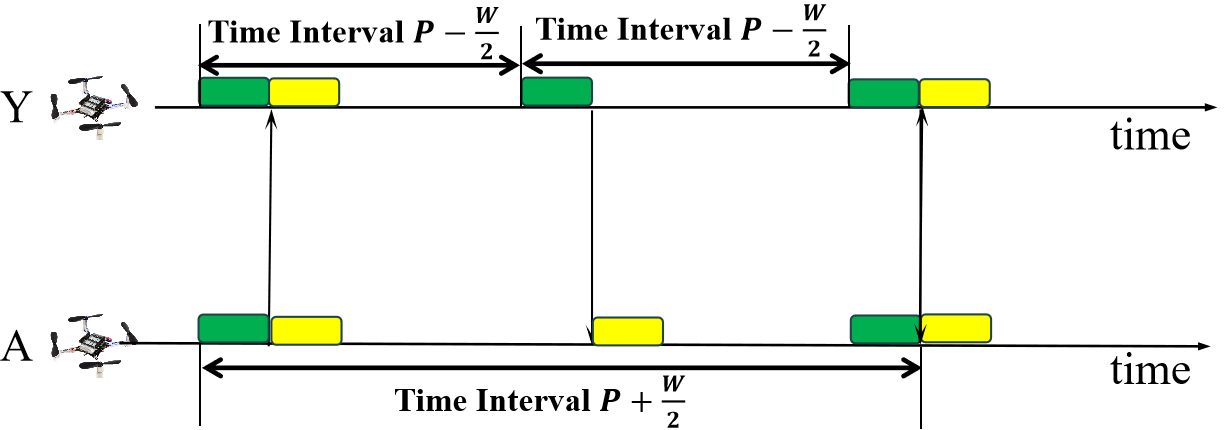
\includegraphics[width=.7\linewidth]{figures/content/chapter3/ProcessTime.png}
  \caption{限制抖动大小的特殊情况}
  \label{fig:3_7}
  \end{figure}
  
当无人机$ A$ 先发送测距报文、随后无人机$Y$ 发送测距报文时，两无人机能够完成一次正常测距。
若在此之后，无人机 $A$ 在无人机$ Y$ 已发送测距报文的情况下再次发送报文，则会发生测距报文不匹配现象。
因此，当条件 $p+w_{A}>p+w_{Y}+\Delta t$成立时，将发生测距报文不匹配。
事件 $ C$ 的发生等价于 $\Delta w>\Delta t$。 
为计算概率 $P(\Delta w> \Delta t)$，首先需要将 $\Delta t$ 的取值范围划分为若干较小的区间，并分别讨论在不同区间内满足条件的 $\Delta t$ 取值范围。
由于必须满足 $\Delta w > \Delta t$，能够满足该条件的 $\Delta t$ 的最大取值为 $W$。
因此，$\Delta t$的取值区间可划分为$\left [ 0,1\right ),\left [ 1,2\right),...,\left[ W-1,W\right)$。
当$\Delta t \in \left [ 0,1\right )$ 时，满足条件的 $\Delta w$取值为 $1,2,...,W$。
同理，当  $\Delta t$ 落入其他区间时，也可以得到相应满足条件的$\Delta w$ 取值范围。
综合上述分析，可最终推导得到事件 $C$ 的发生概率如下所示：
 \begin{equation}
  \begin{aligned}
  P(C)=&\frac{1}{P}\frac{(W+1)W}{2(W+1)^2}+\frac{1}{P}\frac{W(W-1)}{2(W+1)^2}+...+\frac{1}{P}\frac{2}{2(W+1)^2}\\
  =&\frac{1}{2P(W+1)^2}\sum_{k=0}^{W-1}(W+1-k)(W-k) \\
  =&\frac{1}{6P}\frac{W(W^2+3W+2)}{(W+1)^2}
  \end{aligned}
  \end{equation}
因此，我们得到了在对测距周期进行随机化之后，测距不匹配发生的概率。
​\qed

\subsection{权衡测距机制的设计}

尽管通过在测距周期中引入随机性可以显著减少连续测距失败的次数，但该方法也引入了一个新的问题：由于时间戳缺失而导致的测距失败。
当抖动设置过大时，测距周期的波动幅度显著增加，从而更容易引发测距报文不匹配的现象。

如图 \ref{fig:3_8} 所示，当两次测距报文连续发送而且在发送间隔中未接收到来自相邻无人机对应报文的情况下，就会发生消报文不匹配现象。
此时，这些已发送的测距报文缺少测距协议所需的接收时间戳，导致测距过程无法正常完成。
例如，当无人机$A$ 接收到不包含接收时间戳的 $Y_{3}$报文时，与之对应的 $A_{3}$ ​报文的发送时间戳和接收时间戳均未记录在测距表中，从而无法计算最新的测距结果。

\begin{figure}[htbp]
  \centering
  \includegraphics[width=.7\linewidth]{figures/content/chapter3/Problemwithjitter.png}
  \caption{报文不匹配现象}
  \label{fig:3_8}
  \end{figure}

由于时间戳缺失而引起的测距失败，会导致连续测距失败更加频繁且持续时间更长。
该问题源于测距周期的随机化，因此在一定程度上是不可避免的。
所幸的是，我们发现可以通过利用历史时间戳信息来有效缓解这一问题。
在鲁棒集群测距协议中，提出了一种权衡测距方法，用于解决由时间戳缺失导致的测距失败问题。
为此，我们设计了一种新的测距表结构，如图 \ref{fig:3_9} 所示，用以支持权衡测距机制。
在该方法中，当接收到缺失时间戳的测距报文时，系统会调用并使用历史报文中已存储的时间戳来参与距离计算，从而避免测距的失败并降低连续测距失败的发生概率。

在鲁棒集群测距协议中，每完成一次距离计算后，测距表都会进行一次重新整理。 
当接收到报文 $Y_{2}$​ 时，该报文中包含上一条已发送报文$A_{2}$​ 的时间戳，此时可采用 DS-TWR 方法计算当前的最新距离。
若随后接收到不包含接收时间戳的报文 $Y_{3}$ ​ ，则无法继续使用 DS-TWR 完成测距。
然而，此时测距表中已经记录了与报文 $Y_{2}$​ 相关的两个时间戳 $T_{Y_2}$​ 和 $R_{Y_2}$​​ 。 
因此，权衡测距方法会利用报文 $Y_{1}$, $A_{2}$​ 和 $Y_{2}$ ​ 的最近且尚未使用的六个时间戳来完成距离计算，从而弥补时间戳缺失所带来的影响。 
此外，若无人机连续发送多条报文（如 $A_{3}$ 和 $A_{4}$），权衡测距仅保留最新一条报文 $A_{4}$​ 的时间戳。
同样地，当连续接收到多条报文时，下一次发送的测距报文中也仅携带最近一次接收的时间戳。

\begin{figure}[htbp]
  \centering
  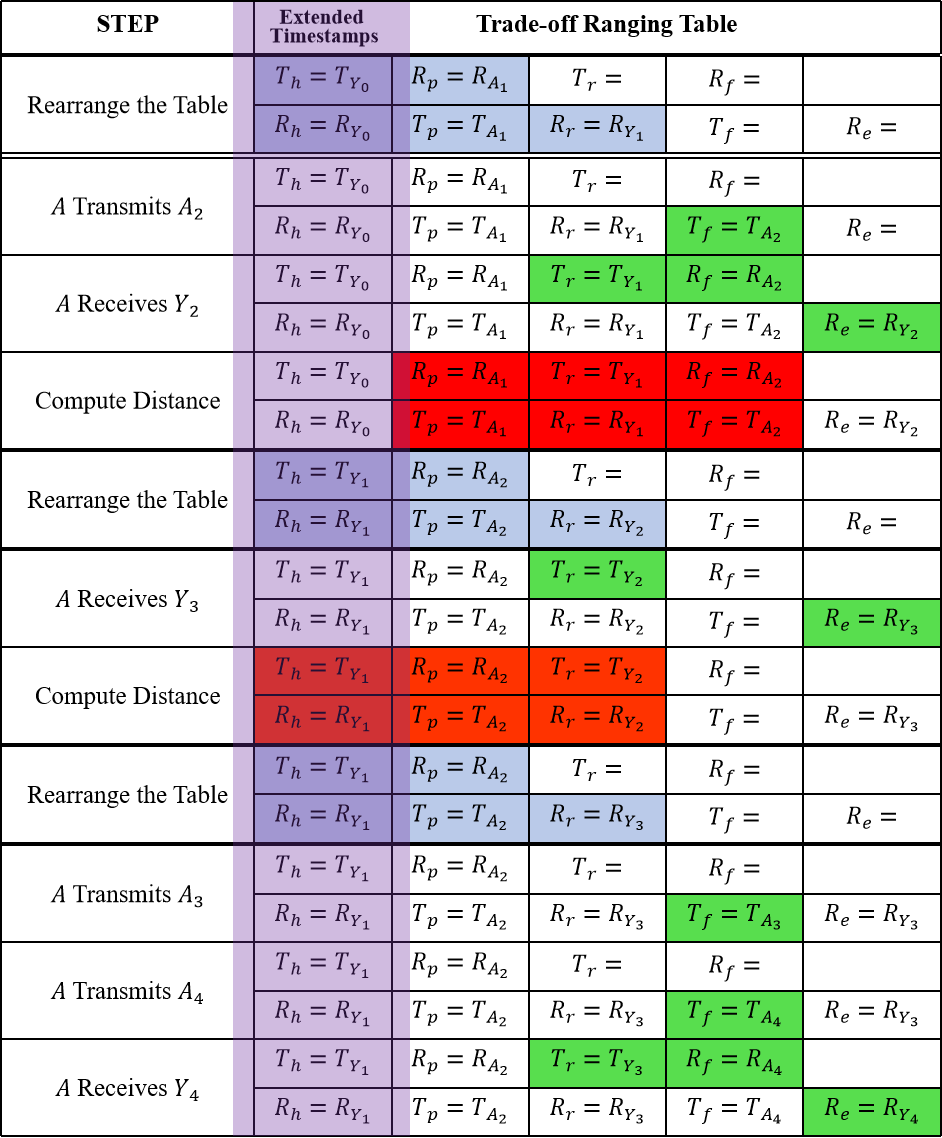
\includegraphics[width=.6\linewidth]{figures/content/chapter3/SwarmRangingSteps.png}
  \caption{采用权衡测距的鲁棒集群测距协议步骤}
  \label{fig:3_9}
\end{figure}

新的测距表结构有效解决了由于时间戳缺失而导致的测距失败问题，其对应的权衡测距方法如算法\ref{alg:trade-off} 所示。

\begin{algorithm}[H]
  \caption{权衡测距算法}
  \label{alg:trade-off}
  \begin{algorithmic}[1]
  
  \While{true}  \Comment{并行任务：发送}
      \State 延时 $P$ 时间
      \ForAll{邻居节点 $Y$}
          \State $Message \gets Message \cup (T_{A_{k-1}}, R_{Y_k})$
      \EndFor
      \State 发送测距报文 $Message$
  \EndWhile
  \Statex
  \Statex \rule{\linewidth}{0.4pt}
  \Statex
  
  \While{true} \Comment{并行任务：接收}
      \State 等待直到接收到测距报文
      \State 设 $Y$ 为报文发送节点的 ID
      \If{在收到的报文中$R_f == \varnothing$}
          \State 对表（AY）：$T_r \gets T_{Y_{k-1}},\; R_f \gets \varnothing,\; R_e \gets R_{Y}$
          \State 利用额外的时间戳计算距离
          \State 更新表：$R_r \gets R_e$（表 AY）
      \Else
          \State 对表（AY）：$T_r \gets T_{Y_{k-1}},\; R_f \gets R_{Y_k},\; R_e \gets R_{Y}$
          \State 计算距离
          \State 更新表：$T_h \gets T_{Y_{k-1}},\; R_h \gets R_{Y_{k-1}},\; R_p \gets R_{A_k},\; T_p \gets T_{A_k},\; R_r \gets R_e$（表 AY）
      \EndIf
  \EndWhile
  
  \end{algorithmic}
\end{algorithm}
      
\subsection{ 最优扰动选择策略}

我们的鲁棒集群测距协议需要在尽可能减少连续测距失败次数的同时，尽量降低权衡测距的发生频率。
因此，本文将该问题建模为一个多目标优化问题，并采用简单加权法来选择合适的抖动参数。
通过在多个目标之间进行协调与折中，实现整体性能的最优。 
在搜索最优抖动参数之前，首先需要对两个目标函数进行归一化处理。
设 $G(W)=1+\frac{1+2W}{W^2+W}$ ,$H(W,P)=P(C)$。
其中，$ G(W)$ 表示连续测距失败次数的度量函数， $H(W,P)$ 表示测距报文不匹配事件发生的概率。
在前文分析中，已将参数$W$ 的取值范围限制为 $\left [ 0, \frac{2}{3}P \right )$。
由于 $G(W)$与 $H(W,P)$ 在该区间内均为单调函数，因此可以分别确定其最大值和最小值。
利用这些极值对目标函数进行归一化，可分别得到归一化后的目标函数 $F_{G}(W)$ 和 $F_{H}(W,P)$。 
据此，本文的多目标优化问题可表示为：


  \begin{equation}
  \begin{aligned}
  \underset{W}{\min }\quad &  \alpha F_{G}(W)+\beta F_{H}(W,P)\\
  \text { s.t. }\quad & 0< W < \frac{2}{3}P\\
  & \alpha + \beta = 1
  \end{aligned}
  \end{equation}

  为有效降低连续测距失败的平均次数，本文将权重系数 $\alpha$设定为 0.9。
  在此权重配置下，得到的最优解 $W^{*}$满足：
  
  \begin{equation}
    \begin{aligned}
    \frac{\partial F(W, P)}{\partial W}=0, F(W,P)=\alpha F_{G}(W)+\beta F_{H}(W) 
    \end{aligned}
    \end{equation} 

根据上述分析，最终可求得最优抖动参数为$W \approx P/10$。
该结果表明，所选取的抖动取值与我们实验章节中的实验结果一致，能够在降低连续测距失败的同时有效抑制测距报文不匹配问题。

\section{自适应协同定位算法}
\subsection{ 系统定义与问题建模}
在进行无人机集群相对定位算法研究之前，本文首先对无人机的机载传感器模型以及无人机相对状态的运动方程进行系统性的介绍，以支撑后续相对定位算法的设计与分析。

\begin{figure}[htbp]
  \centering
  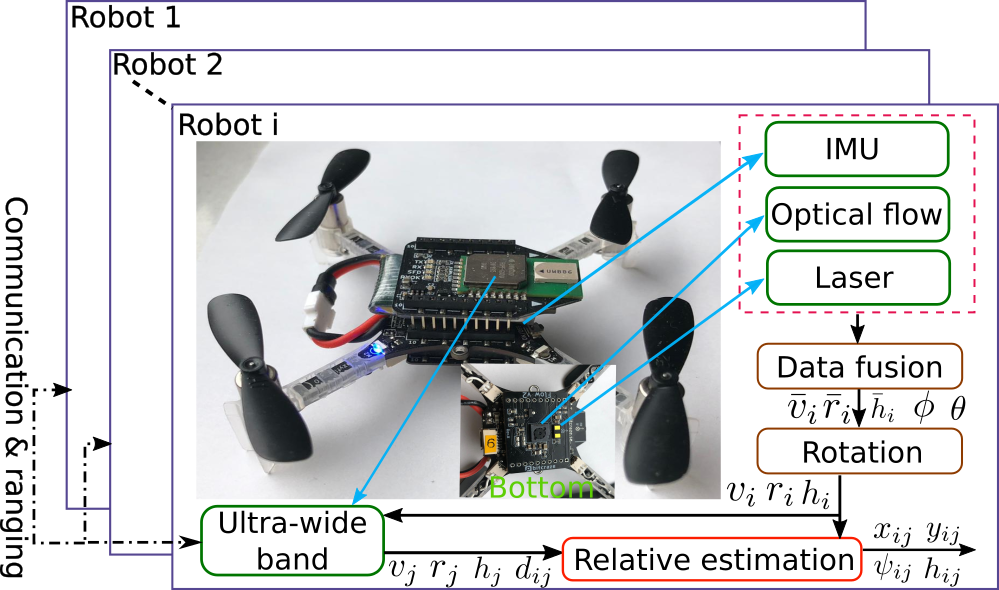
\includegraphics[width=.6\linewidth]{figures/content/chapter3/uwb_sensor.png}
  \caption{无人机集群系统及搭载的机载传感器}
  \label{fig:3_10}
\end{figure}
无人机集群系统中所搭载的传感器如图\ref{fig:3_10}所示。
具体而言，每个无人机均配备惯性测量单元（Inertial Measurement Unit，IMU）、光流传感器以及向下指向的激光测距传感器，用于获取无人机的运动与姿态相关的多源信息。
其中，IMU主要由加速度计和陀螺仪组成，用于测量无人机在本体坐标系下的线加速度和角速度信息。
通过对角速度进行积分可获得无人机的姿态变化情况，而加速度信息则为速度估计和运动建模提供基础，是无人机短时间内高频状态估计的核心传感器。
光流传感器通过观测地面纹理在连续图像帧中的位移变化，估计无人机相对于地面的平移速度，通常用于获取无人机在水平平面内的速度信息。
该传感器不依赖外部定位系统，在近地飞行或低速运动条件下能够提供较为稳定的速度测量，有效抑制仅依赖 IMU 积分所带来的累积误差。
向下指向的激光测距传感器用于测量无人机与地面之间的垂直距离，从而获得高度信息。
该传感器具有测量精度高、响应速度快的特点，可为高度估计提供可靠观测，并与光流传感器协同工作，用于提高速度估计的精度与鲁棒性。

上述传感器数据通过机载滤波器进行融合，得到无人机本体坐标系下的速度、偏航角速率及高度估计值。
随后，利用姿态信息对速度进行坐标变换，将其转换至水平坐标系下，并获得对应的偏航角速率与高度信息。
此外，无人机之间通过超宽带无线通信与测距，基于前文所述的鲁棒集群测距协议实现状态信息的交互与距离测量。
通过融合自身状态估计与来自其他无人机的状态信息，进一步完成对无人机之间相对状态的估计。

为便于分析，本文讨论了任意两个无人机的模型，实现集群协作的前提是无人机$i$需要确定另一个无人机$\{j\mid j\in\mathbb{N}, j\neq i\}$的相对位置。
其中 ， $\mathbb{N}=\{1,2,...,N \}$, $N$是无人机的总数量。
在以无人机$i$为参考坐标系的条件下，定义无人机$j$ 的相对运动状态为 $\boldsymbol{s}_{i j}=\left[\Delta x_{ij}, \Delta y_{i j}, \Delta \theta_{ij}\right]^{\mathrm{T}}$。
结合机载惯性测量单元、光流传感器以及陀螺仪提供的测量信息，可构造系统输入向量$\boldsymbol{u}_{ij}=\left[\boldsymbol{v}_{i}^{\mathrm{T}}, \omega_{i}, \boldsymbol{v}_{j}^{\mathrm{T}}, \omega_{j}\right]^{\mathrm{T}}$。
其中 $\boldsymbol{v}_{i}$​ 与 $\boldsymbol{v}_{j}$分别表示无人机 $i$与 $j$ 在全局参考坐标系下的二维速度向量，
 $\omega_{i}$ ​ 与 $\omega_{j}$ ​ 为对应的偏航角速度。
在牛顿运动定律描述框架下，并仅考虑无人机在水平平面内的平移与偏航运动，可建立无人机对间相对状态的连续时间运动学模型，其表达式为

  \begin{equation}
\dot{\boldsymbol{s}}_{a b}=\boldsymbol{f}\left(\boldsymbol{s}_{a b}, \boldsymbol{u}_{a b}\right)=\left[\begin{array}{c}
\boldsymbol{C}\left(\Delta \theta_{a b}\right) \boldsymbol{v}_{b}-\boldsymbol{v}_{a}-\omega_{a} \boldsymbol{J} \boldsymbol{p}_{a b} \\
\omega_{b}-\omega_{a}
\end{array}\right]
\end{equation}
其中，$\boldsymbol{p}_{a b}=\left[\Delta x_{a b}, \Delta y_{a b}\right]^{\mathrm{T}}$,
$\boldsymbol{C}(\theta)$ 表示二维平面旋转矩阵，$\boldsymbol{J}$ 为二维反对称矩阵，用于刻画角速度对平面位移的耦合影响，其表达式分别为
\begin{equation}
\boldsymbol{C}(\theta)=
\begin{bmatrix}
\cos \theta & -\sin \theta \\
\sin \theta & \cos \theta
\end{bmatrix},
\quad
\boldsymbol{J}=
\begin{bmatrix}
0 & -1 \\
1 & 0  
\end{bmatrix}\text{。}
\end{equation}

基于前文提出的鲁棒集群测距协议，无人机之间可实现相对距离的测量。
设第  $k$  时刻无人机  $i$  与无人机  $j$  的位置分别为
$\boldsymbol{p}_{i, k}=\left[\boldsymbol{x}_{i, k}, \boldsymbol{y}_{i, k}, \boldsymbol{z}_{i, k}\right]^{\mathrm{T}}, \quad \boldsymbol{p}_{j, k}=\left[\boldsymbol{x}_{j, k}, \boldsymbol{y}_{j, k}, \boldsymbol{z}_{j, k}\right]^{\mathrm{T}},$
则无人机  $i$  对无人机  $j$  的距离量测函数可表示为
\begin{equation}
d_{i j, k}=\sqrt{\left(x_{i, k}-x_{j, k}\right)^{2}+\left(y_{i, k}-y_{j, k}\right)^{2}+\left(z_{i, k}-z_{j, k}\right)^{2}} \text{。}
\end{equation}

\subsection{ 自适应扩展卡尔曼滤波算法}
扩展卡尔曼滤波是一类广泛应用于系统状态估计的递推滤波方法，能够处理系统模型中存在的非线性特性以及噪声统计特性未知或近似非高斯的情况。
基于前文构建的无人机状态信息及其运动学模型，本文首先对扩展卡尔曼滤波的预测与校正过程进行说明，随后引入自适应扩展卡尔曼滤波方法，以进一步提升状态估计的鲁棒性与精度。

在采样周期为 $T$ 的条件下，对连续时间模型进行离散化，可得相对状态的离散预测模型为
\begin{equation}
\hat{\mathbf{s}}_{i j, k \mid k-1}=f\left(\hat{\mathbf{s}}_{i j, k-1}, \mathbf{u}_{i j, k-1}\right)=\hat{\mathbf{s}}_{i j, k-1}+\dot{\hat{\mathbf{s}}}_{i j, k-1} T
\end{equation}
其中， $\hat{\mathbf{s}}_{i j, k \mid k-1}$​ 表示在时刻 $ k-1$ 对 $k $时刻的相对状态预测值。

定义相对状态估计误差协方差矩阵为  $\Sigma_{i j, k}$  ，则其预测更新形式为
\begin{equation}
\Sigma_{i j, k \mid k-1}=\Phi_{i j, k-1} \Sigma_{i j, k-1} \Phi_{i j, k-1}^{\mathrm{T}}+\Gamma_{i j, k-1} \Omega_{k-1} \Gamma_{i j, k-1}^{\mathrm{T}}
\end{equation}

其中：
$\Phi_{i j, k}=\left.\frac{\partial f}{\partial \mathbf{s}_{i j}}\right|_{\hat{\mathbf{s}}_{i j, k}}$  为相对运动模型关于状态的雅可比矩阵；
$\Gamma_{i j, k}$  为过程噪声输入矩阵；
$\Omega_{k}$  表示过程噪声协方差矩阵。

在当前预测状态处，对距离观测函数进行一阶泰勒展开，其关于相对状态的雅可比矩阵可表示为
\begin{equation}
J_{i j, k}=\frac{\partial g}{\partial \mathbf{s}_{i j}}=\left[\begin{array}{ccc}
\frac{\Delta x_{i j, k}}{d_{i j, k}} & \frac{\Delta y_{i j, k}}{d_{i j, k}} & 0
\end{array}\right]
\end{equation}
其中，第三项为零是由于距离观测对相对航向角不敏感。

基于预测协方差与观测噪声统计特性，卡尔曼增益矩阵计算如下：
\begin{equation}
G_{i j, k}=\Sigma_{i j, k \mid k-1} J_{i j, k}^{\mathrm{T}}\left(J_{i j, k} \Sigma_{i j, k \mid k-1} J_{i j, k}^{\mathrm{T}}+\Lambda_{k}\right)^{-1}
\end{equation}
其中， $\Lambda_{k}$  为距离测量噪声的协方差矩阵。

在获得距离观测后，相对状态估计可更新为
\begin{equation}
\hat{\mathbf{s}}_{i j, k}=\hat{\mathbf{s}}_{i j, k \mid k-1}+G_{i j, k}\left(d_{i j, k}-g\left(\hat{\mathbf{s}}_{i j, k \mid k-1}\right)\right)
\end{equation}
其中，括号内项为观测残差。

相应的估计误差协方差更新公式为 
\begin{equation}
\begin{array}{l}

\Sigma_{i j, k}=\left(I-G_{i j, k} J_{i j, k}\right) \Sigma_{i j, k \mid k-1}
\end{array}
\end{equation}

在过程噪声协方差矩阵 $\Omega_{k}$ 与观测噪声协方差矩阵$\Lambda_{k}$​ 准确已知的理想条件下，扩展卡尔曼滤波能够为非线性状态空间系统提供线性最小均方误差意义下的最优状态估计。
然而，在实际工程应用中，噪声统计特性往往难以精确获取，一旦 $\Omega_{k}$​ 或 $\Lambda_{k}$ ​ 设定不合理，滤波性能将显著劣化，甚至引发估计不稳定或发散现象。
尤其在微型无人机集群协同定位任务中，由于传感器性能易受环境变化影响，其噪声水平通常具有不确定性和时变性，使得噪声协方差矩阵呈现明显的不确定性与时变特征，从而对定位精度产生不利影响。
因此，研究适用于噪声统计特性不确定条件下的自适应扩展卡尔曼滤波方法具有重要现实意义。 

为进一步阐明噪声协方差矩阵对扩展卡尔曼滤波性能的影响机制，下面对其作用过程进行分析。
当过程噪声协方差矩阵 $\Omega_{k}$​估计不准确时，将首先通过预测协方差更新方程影响相对状态预测误差协方差矩阵$\Sigma_{i j, k\mid ßk−1​}$​的计算结果。
随后，由于卡尔曼增益矩阵$G_{i j, k}$​的求取依赖于$\Sigma_{i j, k\mid ßk−1​}$​，不准确的预测协方差将进一步传递至增益计算过程，最终在状态更新阶段导致相对状态估计$\hat{\mathbf{s}}_{i j, k+1 \mid k}$​偏离最优解，并使对应的估计误差协方差矩阵$\Sigma_{i j, k\mid k−1​}$​失去统计一致性。
因此，过程噪声协方差矩阵$\Omega_{k}$​对滤波性能的影响主要是通过预测误差协方差矩阵$\Sigma_{i j, k\mid ßk−1​}$​间接体现的。

相比之下，观测噪声协方差矩阵$\Lambda_{k}$​ ​的不准确设定将直接作用于卡尔曼增益矩阵$G_{i j, k}$​的计算过程，从而直接影响相对状态的修正结果。
当$\Lambda_{k}$​ ​取值不合理时，将不可避免地导致相对状态估计$\hat{\mathbf{s}}_{i j, k+1 \mid k}$的次优性，并引起估计误差协方差矩阵$\Sigma_{i j, k\mid ßk−1​}$​的不一致问题。
因此，观测噪声协方差矩阵$\Lambda_{k}$​ ​对扩展卡尔曼滤波性能的影响更为直接。

基于上述分析可以看出，相较于难以准确建模的过程噪声协方差矩阵$\Omega_{k}$​，预测误差协方差矩阵$\Sigma_{i j, k\mid k−1​}$​与相对状态估计结果之间具有更加直接的耦合关系，其变化对滤波性能的影响也更为直观，从而为其在线估计与调整提供了可行性。
这一认识构成了本文的主要研究动机。为此，本文提出一种启发式自适应滤波思路，通过对预测误差协方差矩阵$\Sigma_{i j, k\mid k−1​}$​与观测噪声协方差矩阵$\Lambda_{k}$​进行联合估计，避免对过程噪声协方差矩阵$\Omega_{k}$​的直接依赖，并在此基础上设计一种新的自适应扩展卡尔曼滤波算法。

本文旨在利用从初始时刻到当前时刻  $k$  所获得的无人机间距离观测序列$\mathcal{D}_{1: k}=\left\{d_{i j, 1}, d_{i j, 2}, \ldots, d_{i j, k}\right\}$
对预测误差协方差矩阵  $\Sigma_{i j, k \mid k-1}$  以及距离测量噪声协方差矩阵  $\Lambda_{k} $ 进行联合估计。
为此，引入待估参数集合
$\boldsymbol{\theta}_{k} \triangleq\left\{\Sigma_{i j, k \mid k-1}, \Lambda_{k}\right\}$
并基于最大似然准则，通过最大化距离观测序列的对数似然函数$\ell_{\boldsymbol{\theta}_{k}}\left(\mathcal{D}_{1: k}\right) \triangleq \log p_{\boldsymbol{\theta}_{k}}\left(\mathcal{D}_{1: k}\right)$来获得参数估计，即
\begin{equation}
\hat{\boldsymbol{\theta}}_{k}=\arg \max _{\boldsymbol{\theta}_{k}} \ell_{\boldsymbol{\theta}_{k}}\left(\mathcal{D}_{1: k}\right)=\arg \max _{\boldsymbol{\theta}_{k}} \log p_{\boldsymbol{\theta}_{k}}\left(\mathcal{D}_{1: k}\right) 
\end{equation}
其中  $\ell(\cdot)$  表示关于参数  $\boldsymbol{\theta}_{k}$  的对数似然函数。

由于完整联合对数似然函数$\ell_{\boldsymbol{\theta}_{k}}\left(\mathbf{s}_{i j, k}, \mathcal{D}_{1: k}\right) \triangleq \log p_{\boldsymbol{\theta}_{k}}\left(\mathbf{s}_{i j, k}, \mathcal{D}_{1: k}\right)$
相比不完全对数似然函数更易于处理，但相对状态向量  $\mathbf{s}_{i j, k}$  为隐变量，因而上述函数仍不可直接计算。
为此，采用期望最大化思想，通过构造辅助函数
\begin{equation}
\begin{array}{c}
\log p_{\theta_{k}}\left(s_{i j, k}, D_{1: k}\right) \approx \mathcal{Q}\left(\theta_{k}, \theta_{k}^{(l)}\right) \triangleq \mathbb{E}_{s_{i j, k}}\left[\log p_{\theta_{k}}\left(s_{i j, k}, D_{1: k}\right) \mid \theta_{k}^{(l)}, D_{1: k}\right] \\
=\int \log p_{\theta_{k}}\left(s_{i j, k}, D_{1: k}\right) p_{\theta_{k}^{(l)}}\left(s_{i j, k} \mid D_{1: k}\right) d s_{i j, k}
\label{equ:联合概率}
\end{array}
\end{equation}



来近似原对数似然函数，其中  $\theta_{k}^{(l)}$  表示第  $l $ 次迭代的参数估计值。
因此，原始优化问题可转化为$\theta_{k}^{(l+1)} \approx \arg \max _{\theta_{k}} \mathcal{Q}\left(\theta_{k}, \theta_{k}^{(l)}\right)$ 。

下面进行可行性证明：
由联合概率密度函数与条件概率密度函数之间的关系可知，辅助函数的定义式 \ref{equ:联合概率} 可以重新写为：

\begin{equation}
\begin{array}{c}
\mathcal{Q}\left(\theta_{k}, \theta_{k}^{(l)}\right)=\int \log p_{\theta_{k}}\left(s_{i j, k} \mid D_{1: k}\right) p_{\theta_{k}^{(l)}}\left(s_{i j, k} \mid D_{1: k}\right) d s_{i j, k} \\
+\int \log p_{\theta_{k}}\left(D_{1: k}\right) p_{\theta_{k}^{(l)}}\left(s_{i j, k} \mid D_{1: k}\right) d s_{i j, k} \\
=\int \log p_{\theta_{k}}\left(s_{i j, k} \mid D_{1: k}\right) p_{\theta_{k}^{(l)}}\left(s_{i j, k} \mid D_{1: k}\right) d s_{i j, k}+\ell_{\theta_{k}}\left(D_{1: k}\right)
\end{array}
\end{equation}

在上式中令 $\theta_{k}=\theta_{k}^{(l)}$ ，可得：
\begin{equation}
\mathcal{Q}\left(\theta_{k}^{(l)}, \theta_{k}^{(l)}\right)=\int \log p_{\theta_{k}^{(l)}}\left(s_{i j, k} \mid D_{1: k}\right) p_{\theta_{k}^{(l)}}\left(s_{i j, k} \mid D_{1: k}\right) d s_{i j, k}+\ell_{\theta_{k}^{(l)}}\left(D_{1: k}\right)
\end{equation}
因此，
\begin{equation}
 \ell_{\theta_{k}}\left(D_{1: k}\right)-\ell_{\theta_{k}^{(l)}}\left(D_{1: k}\right)=\mathcal{Q}\left(\theta_{k}, \theta_{k}^{(l)}\right)-\mathcal{Q}\left(\theta_{k}^{(l)}, \theta_{k}^{(l)}\right) \\
\int \log \frac{p_{\theta_{k}}\left(s_{i j, k} \mid D_{1: k}\right)}{p_{\theta_{k}^{(l)}}\left(s_{i j, k} \mid D_{1: k}\right)} p_{\theta_{k}^{(l)}}\left(s_{i j, k} \mid D_{1: k}\right) d s_{i j, k}
\end{equation}
由于右侧积分项为 Kullback–Leibler 散度\cite{huang2017novel, tzikas2008variational}，其值非负，因此可得不等式
\begin{equation}
\ell_{\theta_{k}}\left(D_{1: k}\right)-\ell_{\theta_{k}^{(l)}}\left(D_{1: k}\right) \geq \mathcal{Q}\left(\theta_{k}, \theta_{k}^{(l)}\right)-\mathcal{Q}\left(\theta_{k}^{(l)}, \theta_{k}^{(l)}\right) .
\end{equation}
只要保证
$\mathcal{Q}\left(\theta_{k}^{(l+1)}, \theta_{k}^{(l)}\right) \geq \mathcal{Q}\left(\theta_{k}^{(l)}, \theta_{k}^{(l)}\right),$
即可得到$\ell_{\theta_{k}^{(l+1)}}\left(D_{1: k}\right) \geq \ell_{\theta_{k}^{(l)}}\left(D_{1: k}\right),$
从而证明该方法在每次迭代中均能提高对数似然函数值，算法具有可行性与单调收敛性。

下文将基于期望最大化算法进行证明，首先在期望步骤方面：对辅助函数  $\mathcal{Q}\left(\theta_{k}, \theta_{k}^{(l)}\right)$  进行简化。
根据贝叶斯定理，有
\begin{equation}
p_{\theta_{k}}\left(s_{i j, k}, D_{1: k}\right)=p_{\theta_{k}}\left(d_{i j, k} \mid s_{i j, k}\right) p_{\theta_{k}}\left(s_{i j, k} \mid D_{1: k-1}\right) p\left(D_{1: k-1}\right) .
\end{equation}

在扩展卡尔曼滤波框架下，上式中各项可近似表示为高斯分布：
\begin{equation}
\begin{array}{c}
p_{\theta_{k}}\left(s_{i j, k} \mid D_{1: k-1}\right)=\mathcal{N}\left(s_{i j, k} ; \hat{s}_{i j, k \mid k-1}, \Sigma_{i j, k \mid k-1}\right) \\
p_{\theta_{k}}\left(d_{i j, k} \mid s_{i j, k}\right)=\mathcal{N}\left(d_{i j, k} ; g\left(s_{i j, k}\right), \Lambda_{k}\right)
\end{array}
\end{equation}

由于  $p\left(D_{1: k-1}\right)$  与参数  $\theta_{k}$  无关，因此在最大化过程中可视为常数项。
于是，对数联合概率密度函数可写为
\begin{equation}
\log p_{\theta_{k}}\left(s_{i j, k}, D_{1: k}\right)=-\frac{1}{2} \log \left|\Lambda_{k}\right|-\frac{1}{2}\left(d_{i j, k}-g\left(s_{i j, k}\right)\right)^{T} \Lambda_{k}^{-1}\left(d_{i j, k}-g\left(s_{i j, k}\right)\right)+c_{\theta_{k}} .
\end{equation}

进一步近似后验分布为
\begin{equation}
p_{\theta_{k}}^{(l)}\left(s_{i j, k} \mid D_{1: k}\right)=\mathcal{N}\left(s_{i j, k} ; \hat{s}_{i j, k \mid k}^{(l+1)}, \Sigma_{i j, k \mid k}^{(l+1)}\right) .
\end{equation}
将上述结果代入辅助函数，可得

\begin{equation}
\mathcal{Q}\left(\theta_{k}, \theta_{k}^{(l)}\right)=-\frac{1}{2} \log \left|\Lambda_{k}\right|-\frac{1}{2} \operatorname{tr}\left(A_{k} \Lambda_{k}^{-1}\right)-\frac{1}{2} \log \left|\Sigma_{i j, k \mid k-1}\right|-\frac{1}{2} \operatorname{tr}\left(B_{k} \Sigma_{i j, k \mid k-1}^{-1}\right)+c_{\theta_{k}},
\end{equation}

其中
\begin{equation}
\begin{aligned}
A_{k} & =\int\left[d_{i j, k}-g\left(s_{i j, k}\right)\right]\left[d_{i j, k}-g\left(s_{i j, k}\right)\right]^{T} \mathcal{N}\left(s_{i j, k} ; \hat{s}_{i j, k \mid k}^{(l+1)}, \Sigma_{i j, k \mid k}^{(l+1)}\right) d s_{i j, k} \\
B_{k} & =\int\left(s_{i j, k}-\hat{s}_{i j, k \mid k-1}\right)\left(s_{i j, k}-\hat{s}_{i j, k \mid k-1}\right)^{T} \mathcal{N}\left(s_{i j, k} ; \hat{s}_{i j, k \mid k}^{(l+1)}, \Sigma_{i j, k \mid k}^{(l+1)}\right) d s_{i j, k}
\end{aligned}
\end{equation}

根据上文定义的距离观测模型，在当前迭代估计点 $\hat{s}_{i j, k}^{(l+1)}$处对观测函数进行一阶泰勒展开，可得
\begin{equation}
g\left(s_{i j, k}\right) \approx g\left(\hat{s}_{i j, k}^{(l+1)}\right)+J_{i j, k}^{(l+1)}\left(s_{i j, k}-\hat{s}_{i j, k}^{(l+1)}\right)
\end{equation}
其中,$J_{i j, k}^{(l+1)}=\left.\frac{\partial g}{\partial s_{i j}}\right|_{\hat{s}_{i j, k}^{(l+1)}}$表示观测函数在  $\hat{s}_{i j, k}^{(l+1)}$  处的雅可比矩阵。
根据距离函数的偏导计算，可得$J_{i j, k}^{(l+1)}=\left[\begin{array}{ll}
\frac{\Delta x_{i j, k}}{d_{i j, k}} & \frac{\Delta y_{i j, k}}{d_{i j, k}}
\end{array}\right]$
利用线性化的结果对$A_{k} $和$B_{k}$进行详细的推导计算：
利用上述的线性化结果代入可得
\begin{equation}
\begin{aligned}
A_{i j, k}= & \int\left[d_{i j, k}-g\left(\hat{s}_{i j, k \mid k}^{(l+1)}\right)-J_{i j, k}^{(l+1)}\left(s_{i j, k}-\hat{s}_{i j, k \mid k}^{(l+1)}\right)\right] \\
& {\left[d_{i j, k}-g\left(\hat{s}_{i j, k \mid k}^{(l+1)}\right)-J_{i j, k}^{(l+1)}\left(s_{i j, k}-\hat{s}_{i j, k \mid k}^{(l+1)}\right)\right]^{T} } \\
& \mathcal{N}\left(s_{i j, k} ; \hat{s}_{i j, k \mid k}^{(l+1)}, \Sigma_{i j, k \mid k}^{(l+1)}\right) d s_{i j, k}
\end{aligned}
\end{equation}

利用高斯积分公式可得
\begin{equation}
A_{i j, k}=\left[d_{i j, k}-g\left(\hat{s}_{i j, k \mid k}^{(l+1)}\right)\right]\left[d_{i j, k}-g\left(\hat{s}_{i j, k \mid k}^{(l+1)}\right)\right]^{T}+J_{i j, k}^{(l+1)} \Sigma_{i j, k \mid k}^{(l+1)}\left(J_{i j, k}^{(l+1)}\right)^{T}
\end{equation}

同理可得：
\begin{equation}
\begin{aligned}
B_{i j, k}=\int & \left(s_{i j, k}-\hat{s}_{i j, k \mid k}^{(l+1)}+\hat{s}_{i j, k \mid k}^{(l+1)}-\hat{s}_{i j, k \mid k-1}\right) \\
& \left(s_{i j, k}-\hat{s}_{i j, k \mid k}^{(l+1)}+\hat{s}_{i j, k \mid k}^{(l+1)}-\hat{s}_{i j, k \mid k-1}\right)^{T} \\
& \mathcal{N}\left(s_{i j, k} ; \hat{s}_{i j, k \mid k}^{(l+1)}, \Sigma_{i j, k \mid k}^{(l+1)}\right) d s_{i j, k}
\end{aligned}
\end{equation}

最终得到
\begin{equation}
B_{i j, k}=\Sigma_{i j, k \mid k}^{(l+1)}+\left(\hat{s}_{i j, k \mid k}^{(l+1)}-\hat{s}_{i j, k \mid k-1}\right)\left(\hat{s}_{i j, k \mid k}^{(l+1)}-\hat{s}_{i j, k \mid k-1}\right)^{T}
\end{equation}

在最大化步骤中，通过最大化  $\mathcal{Q}\left(\theta_{k}, \theta_{k}^{(l)}\right)$  对参数  $\theta_{k}$  进行更新，即
\begin{equation}
\left.\frac{\partial \mathcal{Q}\left(\theta_{k}, \theta_{k}^{(l)}\right)}{\partial \theta_{k}}\right|_{\theta_{k}=\theta_{k}^{(l+1)}}=0 .
\end{equation}

由于$\theta_{k}=\left\{\Sigma_{i j, k \mid k-1}, \Lambda_{k}\right\},$上述条件可分别转化为
\begin{equation}
\frac{\partial \mathcal{Q}}{\partial \Sigma_{i j, k \mid k-1}}=0, 
\frac{\partial \mathcal{Q}}{\partial \Lambda_{k}}=0 .
\end{equation}


偏导数$\frac{\partial \mathcal{Q}\left(\theta_{k}, \theta_{k}^{(l)}\right)}{\partial \Sigma_{i j, k \mid k-1}}$
和$\frac{\partial \mathcal{Q}\left(\theta_{k}, \theta_{k}^{(l)}\right)}{\partial \Lambda_{k}}$
可以被计算如下：
\begin{equation}
\begin{array}{c}
\frac{\partial \mathcal{Q}\left(\theta_{k}, \theta_{k}^{(l)}\right)}{\partial \Sigma_{i j, k \mid k-1}}=-\frac{1}{2} \Sigma_{i j, k \mid k-1}^{-1}+\frac{1}{2} \Sigma_{i j, k \mid k-1}^{-1} B_{k} \Sigma_{i j, k \mid k-1}^{-1} \\
\frac{\partial \mathcal{Q}\left(\theta_{k}, \theta_{k}^{(l)}\right)}{\partial \Lambda_{k}}=-\frac{1}{2} \Lambda_{k}^{-1}+\frac{1}{2} \Lambda_{k}^{-1} A_{k} \Lambda_{k}^{-1}
\end{array}
\end{equation}

因此求解可得更新公式
\begin{equation}
\Sigma_{i j, k \mid k-1}^{(l+1)}=B_{k},  \Lambda_{k}^{(l+1)}=A_{k}
\end{equation}

\begin{figure}[htbp]
  \centering
  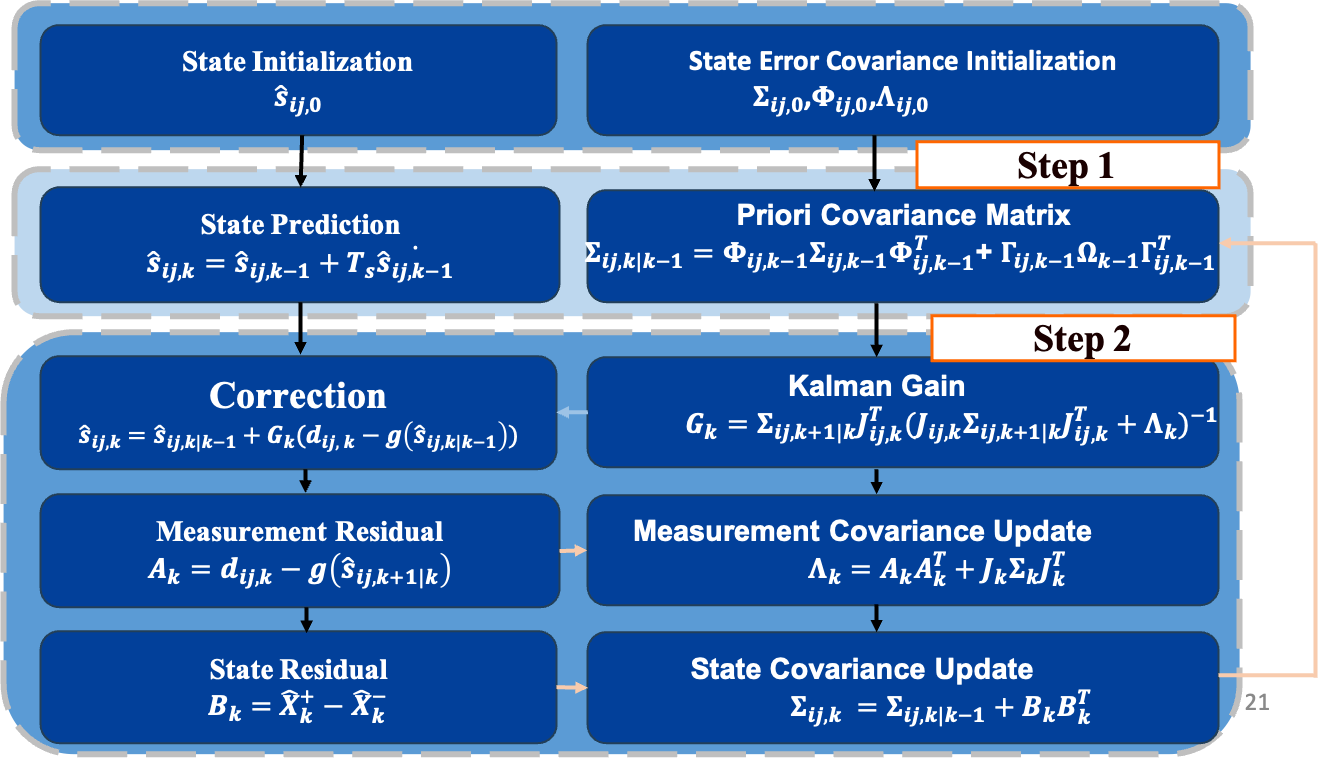
\includegraphics[width=.8\linewidth]{figures/content/chapter3/自适应EKF算法流程.png}
  \caption{自适应扩展卡尔曼滤波算法流程图}
  \label{fig:3_11}
\end{figure}

上述为所提出自适应扩展卡尔曼滤波算法的可行性证明，算法伪代码如算法\ref{alg:AEKF_UAV} 所示。


针对传统扩展卡尔曼滤波在实际应用中对过程噪声协方差和观测噪声协方差依赖性较强、相关参数难以准确获取的问题，本章在原有滤波框架基础上，引入期望最大化算法构建参数自适应估计机制。
具体而言，将预测误差协方差矩阵与观测噪声协方差矩阵视为待估参数。在期望步中，通过计算完全数据对数似然函数的条件期望来估计隐藏变量的统计特性；
在最大化步中，对上述期望函数进行极大化求解，从而得到参数的更新表达式。
基于该过程，推导获得了预测协方差矩阵和观测噪声协方差矩阵的递推更新公式，并将其嵌入扩展卡尔曼滤波的迭代计算流程中，形成一种自适应扩展卡尔曼滤波算法。

通过上述方法，所提出的自适应扩展卡尔曼滤波能够在噪声统计特性未知或存在不确定性的情况下，实现对无人机相对状态的稳定估计。
同时，该方法能够根据观测数据动态调整噪声参数，提高滤波算法对环境变化的适应能力，从而为无人机协同定位与编队控制提供一种有效且鲁棒的状态估计方案。


\begin{algorithm}[H]
\caption{基于期望最大化算法的自适应扩展卡尔曼滤波算法}
\label{alg:AEKF_UAV}

\begin{algorithmic}

\State \textbf{输入：}  $\hat{s}_{ij,k-1|k-1}$， $\Sigma_{ij,k-1|k-1}$，$\Omega_{k-1}$, $\mathbf{u}_{ij, k}$， $g(s_{ij,k})$，
 $d_{ij,k}$，$\tilde{\Sigma}_{ij,k-1}$，
$\tilde{\Lambda}_{k-1}$，$N$

\State \textbf{时间更新：}

\State 1. $\hat{\mathbf{s}}_{i j, k \mid k-1}=\hat{\mathbf{s}}_{i j, k-1}+\dot{\hat{\mathbf{s}}}_{i j, k-1} T$


\State 2. $\Sigma_{i j, k \mid k-1}=\Phi_{i j, k-1} \Sigma_{i j, k-1} \Phi_{i j, k-1}^{\mathrm{T}}+\Gamma_{i j, k-1} \Omega_{k-1} \Gamma_{i j, k-1}^{\mathrm{T}}$

\State \textbf{迭代测量更新：}

\State 3. 初始化：$\Sigma^{(0)}_{ij,k|k-1} = \tilde{\Sigma}_{ij,k|k-1},\quad \Lambda^{(0)}_k = \tilde{\Lambda}_k$, $\hat{s}^{(0)}_{ij,k|k} = \hat{s}_{ij,k|k-1}$

\For{$l = 0 : N - 1$}

\State 给定 $\Sigma^{(l)}_{ij,k|k-1}$、$\Lambda^{(l)}_k$ 和 $\hat{s}^{(l)}_{ij,k|k}$，更新 $\hat{s}^{(l+1)}_{ij,k|k}$ 和 $\Sigma^{(l+1)}_{ij,k|k}$：

\State 4. 计算雅可比矩阵
\[
J^{(l)}_{ij,k} =
\begin{bmatrix} 
\dfrac{\Delta x^{(l)}_{ij,k|k}}{\sqrt{(\Delta x^{(l)}_{ij,k|k})^2 + (\Delta y^{(l)}_{ij,k|k})^2}}, &
\dfrac{\Delta y^{(l)}_{ij,k|k}}{\sqrt{(\Delta x^{(l)}_{ij,k|k})^2 + (\Delta y^{(l)}_{ij,k|k})^2}}
\end{bmatrix}
\]

\State 5. 计算卡尔曼增益: $G^{(l+1)}_{ij,k} =
\Sigma^{(l)}_{ij,k|k-1}(J^{(l)}_{ij,k})^T
\left(
J^{(l)}_{ij,k}\Sigma^{(l)}_{ij,k|k-1}(J^{(l)}_{ij,k})^T + \Lambda^{(l)}_k
\right)^{-1}$

\State 6. 更新状态估计:$
\hat{s}^{(l+1)}_{ij,k|k}
=
\hat{s}_{ij,k|k-1}
+
G^{(l+1)}_{ij,k}
\left(
d_{ij,k}
-
g(\hat{s}^{(l)}_{ij,k|k})
-
J^{(l)}_{ij,k}
(\hat{s}_{ij,k|k-1} - \hat{s}^{(l)}_{ij,k|k})
\right)
$

\State 7. 更新后验协方差:$
\Sigma^{(l+1)}_{ij,k|k}
=
\Sigma^{(l)}_{ij,k|k-1}
-
G^{(l+1)}_{ij,k}
J^{(l)}_{ij,k}
\Sigma^{(l)}_{ij,k|k-1}
$

\State 8. 计算更新后的雅可比矩阵
\[
J^{(l+1)}_{ij,k} =
\begin{bmatrix} 
\dfrac{\Delta x^{(l+1)}_{ij,k|k}}{\sqrt{(\Delta x^{(l+1)}_{ij,k|k})^2 + (\Delta y^{(l+1)}_{ij,k|k})^2}}, &
\dfrac{\Delta y^{(l+1)}_{ij,k|k}}{\sqrt{(\Delta x^{(l+1)}_{ij,k|k})^2 + (\Delta y^{(l+1)}_{ij,k|k})^2}}
\end{bmatrix}
\]

\State 9. 计算观测相关矩阵:
$A_k =
\left[d_{ij,k} - g(\hat{s}^{(l+1)}_{ij,k|k})\right]
\left[d_{ij,k} - g(\hat{s}^{(l+1)}_{ij,k|k})\right]^T
+
J^{(l+1)}_{ij,k}
\Sigma^{(l+1)}_{ij,k|k}
(J^{(l+1)}_{ij,k})^T$


\State 10. 计算状态相关矩阵:
\[B_k =
\Sigma^{(l+1)}_{ij,k|k}
+
(\hat{s}^{(l+1)}_{ij,k|k} - \hat{s}_{ij,k|k-1})
(\hat{s}^{(l+1)}_{ij,k|k} - \hat{s}_{ij,k|k-1})^T
\]

\State 11. 更新参数:
$\Sigma^{(l+1)}_{ij,k|k-1} = B_k,\quad
\Lambda^{(l+1)}_k = A_k$


\EndFor

\State 12. 输出最终估计结果
\[
\hat{s}_{ij,k|k} = \hat{s}^{(N)}_{ij,k|k},\quad
\Sigma_{ij,k|k} = \Sigma^{(N)}_{ij,k|k},\quad
\hat{\Sigma}_{ij,k|k-1} = \Sigma^{(N)}_{ij,k|k-1},\quad
\hat{\Lambda}_k = \Lambda^{(N)}_k
\]

\State \textbf{输出：} 当前时刻后验状态估计 $\hat{s}_{ij,k|k}$，后验协方差 $\Sigma_{ij,k|k}$，
预测协方差估计 $\hat{\Sigma}_{ij,k|k-1}$ 和观测噪声协方差估计 $\hat{\Lambda}_k$

\end{algorithmic}

\end{algorithm}

\section{实验设置与结果分析}

本节通过真实无人机集群实验，对所提出的鲁棒集群测距协议以及自适应协同定位算法的实际性能进行验证，并进一步展示在仅依赖相对定位信息条件下的大规模无人机集群自主飞行能力。

实验平台采用商业微型四旋翼无人机 Crazyflie 2.1 构建无人机集群系统。
如图\ref{fig:3_12}所示，每架无人机均搭载多种传感器模块，用于实现相对定位与集群飞行。具体配置如下：

\begin{figure}[htbp]
  \centering
  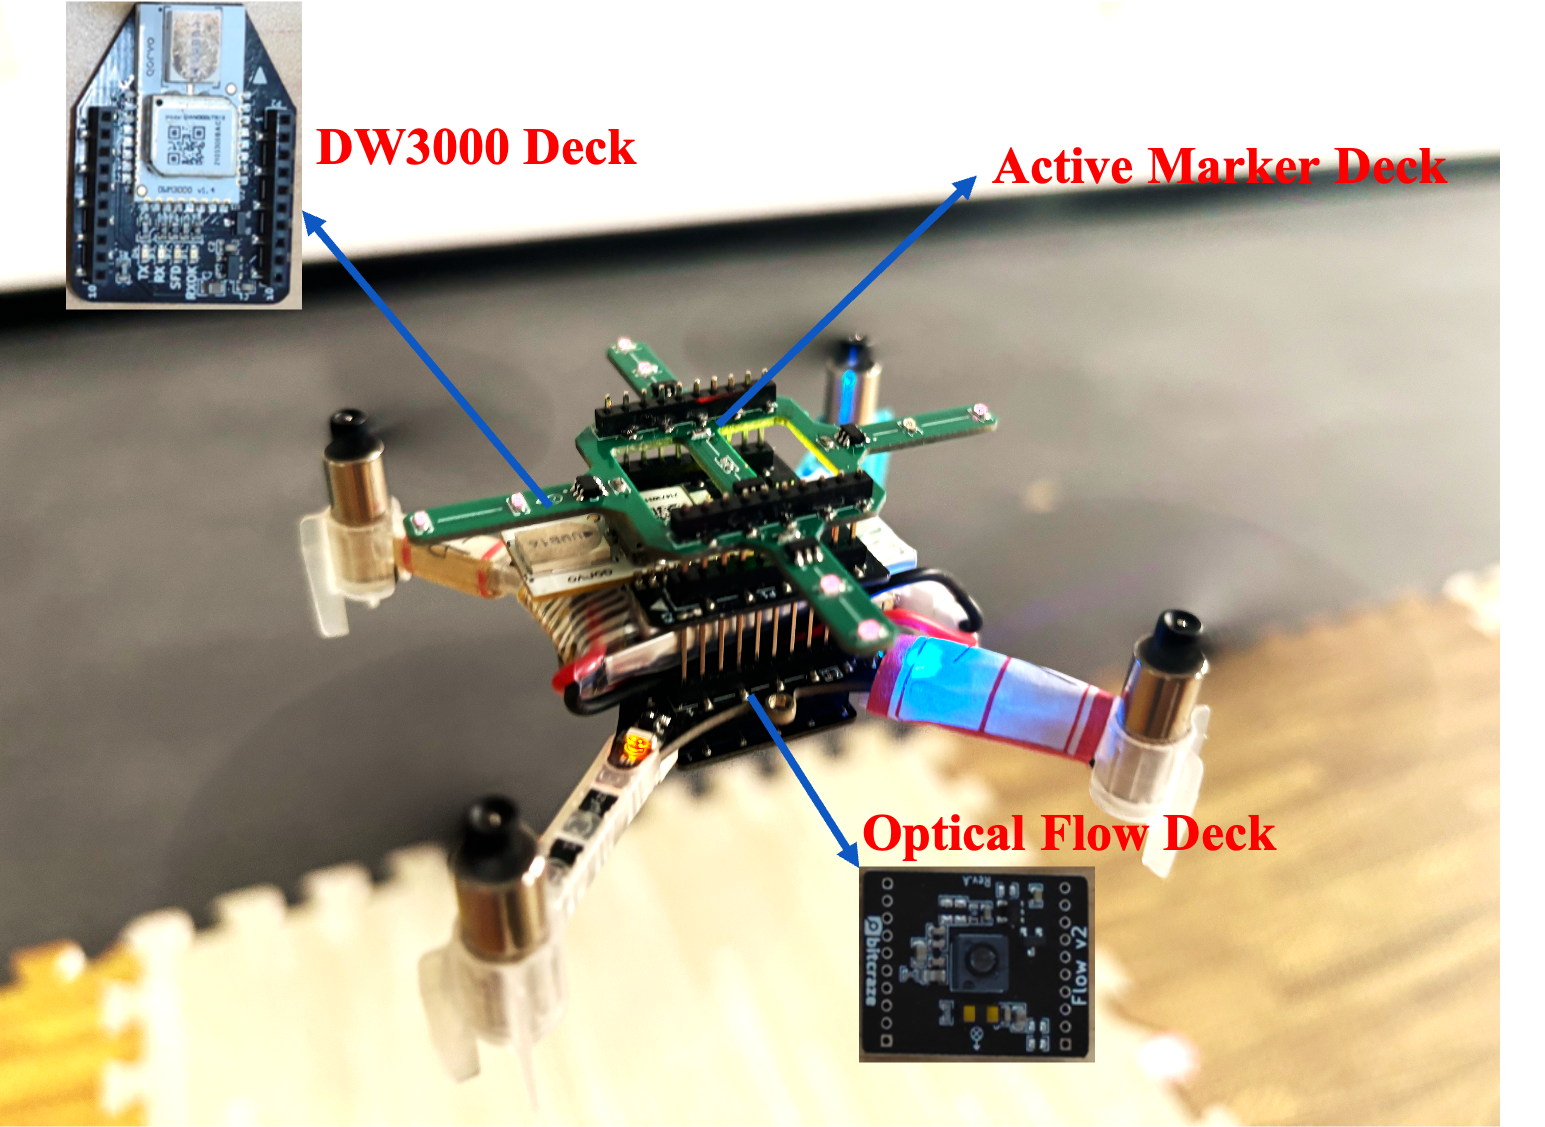
\includegraphics[width=.6\linewidth]{figures/content/chapter3/crazyflie_drone_flo_uwb.pdf}
  \caption{实验用到的无人机以及传感器}
  \label{fig:3_12}
\end{figure}

\begin{itemize}
\item 惯性测量单元（IMU）：包含三轴加速度计和三轴陀螺仪，用于获取无人机的姿态和运动信息。

\item 光流传感器模块（Optical Flow Deck）：由 VL53L1x 激光高度传感器和 PMW3901 光流传感器组成，可提供最高 100 Hz 的速度测量数据。

\item 超宽带测距模块（UWB3000 Deck）：基于 DWM3000 UWB芯片，用于无人机之间的距离测量，是实现集群相对定位的重要信息来源。

\item 主动标记模块（Active Marker Deck）：由高功率 LED 构成，可设置不同 ID，从而在运动捕捉系统中实现大量刚体目标的唯一识别，避免使用大量反光标记。
\end{itemize}

无人机系统采用STM32F4微控制器作为主处理单元，主频 168 MHz，片上内存 192 KB。
在该处理器上同时运行的核心算法模块包括：集群测距协议、自适应相对定位算法与飞行控制算法。

所有实验均在 6 m × 6 m 的室内实验场地中进行，如图\ref{fig:3_13}所示。
为了获得精确的参考数据，实验系统使用 OptiTrack运动捕捉系统实时获取每架无人机的真实位置与偏航角。
该系统提供高精度位姿信息，用于记录实验真实轨迹并在实验后进行性能评估与误差分析
需要说明的是，运动捕捉系统数据仅用于实验结果验证和后期数据分析，并未参与算法的在线估计过程。无人机在实际运行过程中仅依赖机载传感器和UWB测距信息进行相对定位与协同飞行。

\begin{figure}[htbp]
  \centering
  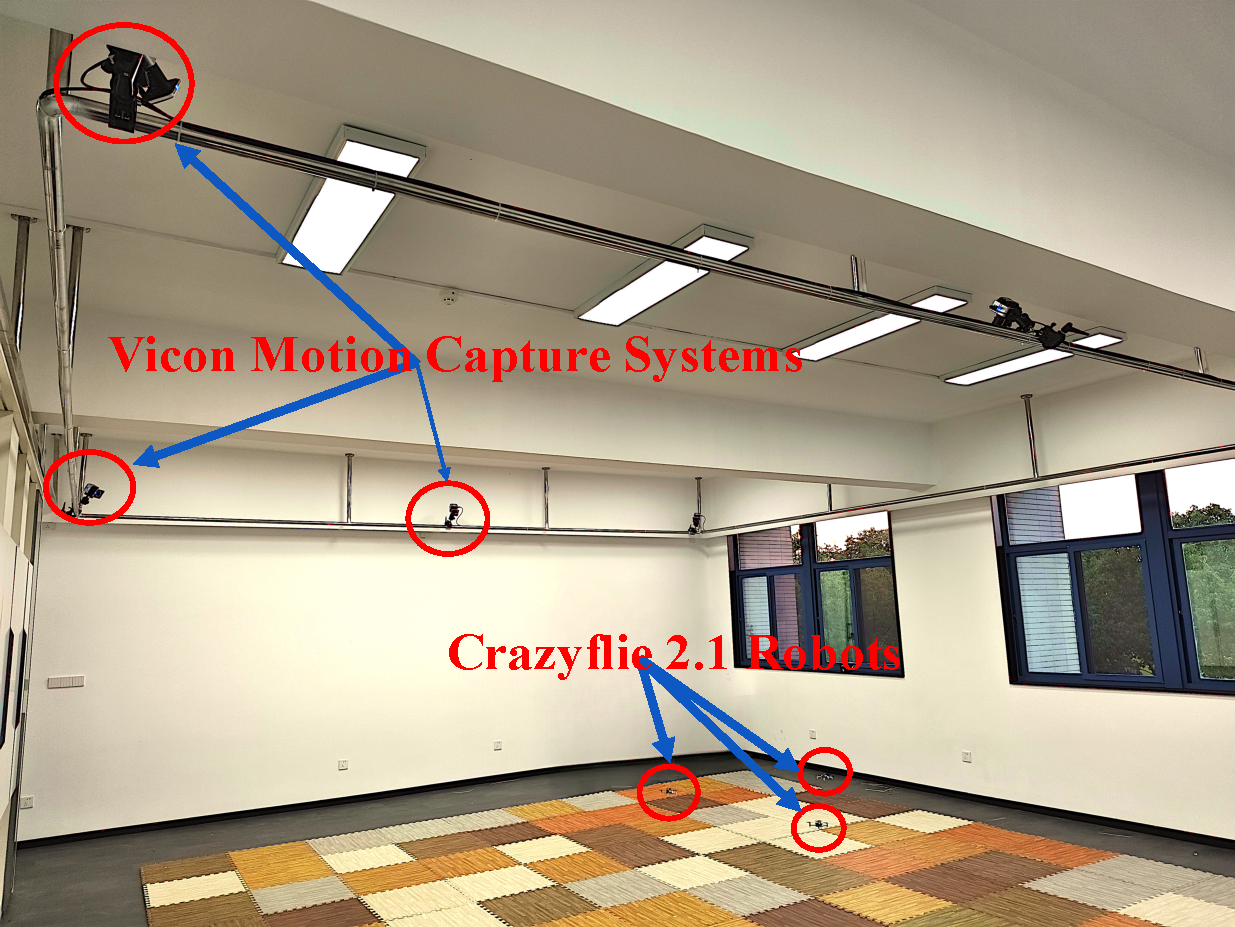
\includegraphics[width=.6\linewidth]{figures/content/chapter3/environment.pdf}
  \caption{实验场地}
  \label{fig:3_13}
\end{figure}


通过大量真实飞行实验验证，所提出的鲁棒集群测距协议能够在动态密集的无人机网络环境中提供稳定、高效的距离更新，从而显著提升自适应协同定位算法在大规模无人机集群中的定位性能与鲁棒性。

\subsection{  DW3000的时钟偏移与处理时间验证}

为研究两块 DW3000 芯片之间的时钟偏差，本小节设计并开展了一组实验。
在该实验中，两个无人机同时按照 10 ms 的测距周期执行周期性测距任务，并记录了 10,000 次消息发送的时间戳。

实验结果表明，两无人机的平均测距周期分别为 9.981966 ms 和 9.988414 ms。
由此可以得到，两无人机发送报文的时间戳差值（即两块 DW3000 芯片之间的相对时钟偏差）约为 0.00645 ms（即 9.988414 ms − 9.981966 ms）。
尽管该时钟偏差数值较小，但随着时间累积会导致同步误差的逐渐增大。
具体而言，在约 15.5 s 之后（计算方式为 10 ms x 10ms/ 0.00645 ms），两无人机将进入连续测距失败阶段。

此外，还开展了另一组实验以评估 DW3000 芯片处理报文的时间开销。
在该实验中，通过计算无人机发送报文后与下一次接收报文的时间戳差值，连续两次接收报文时间戳之间的差值来估计芯片在发送和接收报文过程中的处理时间。
实验过程中未为无人机设置随机化等待时间。
在时钟偏差的影响下，所测得的时间差会从一个最小值逐渐增加至最大值，其中最小值对应于芯片完成一次报文发送和接收所需的处理时间，而最大值对应于测距周期。

实验结果如 表 \ref{tab:timing} 所示。结果表明，即使在 26 架机器人组成的集群系统中，单条测距消息的处理时间仍然 小于 1 ms。
实验数据可以进一步被用于第 \ref{sec:sim_performence}节中的仿真实验参数设置。

\begin{table}[h]
\centering
\caption{不同规模无人机集群中的报文收发处理时间}
\label{tab:timing}
\begin{tabular}{|c|c|c|c|c|}
\hline
\textbf{集群数量} & 2   & 10  & 18  & 26  \\ \hline
\textbf{报文发送处理时间}               & 0.167ms & 0.259ms & 0.312ms & 0.389ms \\ \hline
\textbf{报文接收处理时间}               & 0.339ms & 0.441ms & 0.548ms & 0.662ms \\ \hline
\end{tabular}
\end{table}
\subsection{ 大规模集群测距的仿真鲁棒性分析}
\label{sec:sim_performence}

前文已从理论角度分析了两架无人机执行鲁棒集群测距协议时的性能表现。
然而，在大规模无人机集群中，随着参与无人机数量的增加，集群内部的通信与测距交互显著增多，同时信号干扰的可能性也随之提高，从而使系统复杂度大幅上升。
因此，在包含大量无人机参与的场景下，对鲁棒集群测距协议性能进行建模与预测成为一项具有挑战性的任务。
为此，本节通过构建仿真模型，对大规模集群环境下该协议的性能进行分析。

\begin{algorithm}[htbp]
\caption{大规模集群收发包仿真算法}
\label{alg:sim_alg}
\setlength{\baselineskip}{0.98\baselineskip}
\textbf{Input:} $N, P, W, D, I$ \\
\textbf{Output:} $recv\_packets$ \\
$packets = generateTxPacket(N, P, W, D)$ \\
计算 $tx, rx$ by Eq.(\ref{eq:txrxdiff}) and (\ref{eq:rxtxdiff}) \\
初始化 $recv\_packets = [\,]$ and $seq = 1$ \\
\textbf{for} $pkt$ in $packets$ \textbf{do} \\
\hspace*{1em} \textbf{if} $pkt.id == I$ \textbf{then} \\
\hspace*{1em} $tran\_Start = pkt.tx,\; tran\_End = pkt.tx + tx,\; seq++$ \\
\hspace*{1em} \textbf{continue} \\
\hspace*{1em} \textbf{end if} \\
\hspace*{1em} \textbf{if} $pkt.tx \ge rece\_Start$ and $pkt.tx \le rece\_End$ \textbf{then} \\
\hspace*{1em} \textbf{continue} \\
\hspace*{1em} \textbf{end if} \\
\hspace*{1em} \textbf{if} $pkt.tx \ge tran\_Start$ and $pkt.tx \le tran\_End$ \textbf{then} \\
\hspace*{1em} \textbf{continue} \\
\hspace*{1em} \textbf{end if} \\
\hspace*{1em} \textbf{if} $packets[I][seq].tx \le pkt.tx \le packets[I][seq].tx + tx$ \textbf{then} \\
\hspace*{1em} \textbf{continue} \\
\hspace*{1em} \textbf{end if} \\
\hspace*{1em} $rece\_Start = pkt.tx + tx,\; rece\_End = pkt.tx + rx$ \\
\hspace*{1em} $recv\_packets.append(pkt)$ \\
\textbf{end for}

\end{algorithm}

仿真工具的核心功能是模拟目标无人机发送数据包以及从邻居无人机接收数据包的过程，并考虑数据报文在传输过程中可能发生的丢失情况。
该仿真工具的输入参数包括：用于仿真的无人机数量 $N$、测距周期的平均值$P$、测距周期的抖动范围 $W$、
目标无人机编号 $I$，以及总仿真时长$D$。

在仿真过程中，一个关键挑战在于如何合理地设置各无人机之间的时钟偏差。
为此，利用真实实验中测得的测距周期的均值和方差，为每架无人机随机生成一系列数据报文的发送时间戳，以模拟真实系统中的时钟漂移特性。

为了模拟目标无人机从邻居无人机接收报文的过程，需要对报文发送与接收过程中的处理时间进行精确建模。
当接收操作与另一接收操作或发送操作之间的时间间隔过小时，接收过程可能发生失败。
因此，在仿真模型中需要考虑报文发送与接收处理时间之间的约束关系。

此外，为了刻画报文大小与处理时间之间的关系，采用线性回归分析方法建立相应的线性模型。该线性函数可以表示为：
\begin{align}
tx &= tx\_k * packetSize + tx\_b, \label{eq:txrxdiff}\\
rx &= rx\_k * packetSize + rx\_b, \label{eq:rxtxdiff}
\end{align}
其中，模型参数通过最小二乘法进行估计，不同数据包大小对应的处理时间如表\ref{tab:timing}所示。

该算法的核心思想是判断无人机是否能够成功接收数据包。
仿真核心部分的伪代码如算法 \ref{alg:sim_alg}所示。
在仿真过程中，按照时间顺序依次遍历每一个数据包，并根据模拟得到的处理时间判断该数据包是否应被丢弃。
如果某一邻居无人机在其自身发送或接收报文的处理时间内发送数据包，则该数据包将被判定为丢失。
通过对无人机集群中的报文发送与接收过程进行仿真，并结合前述分析，可以进一步判断系统中是否出现连续测距失败或权衡测距的情况。

图 \ref{fig:3_14}展示了仿真实验结果。
仿真分别在 25、50、75 和 100 架无人机组成的集群规模下进行，仿真时长为 200 s，平均测距周期设置为 100 ms。
实验结果表明，随着集群规模的增大，由于报文大小增加以及丢失概率上升，系统中出现连续测距失败的次数也随之增加。
此外，随着随机化程度的提高，连续测距失败的平均次数呈现下降趋势。
值得注意的是，权衡测距的比例基本不受集群规模影响，而仅与随机数的选择有关。
上述结果验证了该协议在大规模集群场景下的可扩展性，并为其在实际系统中的部署提供了参考依据。

\begin{figure}[h]
\centerline{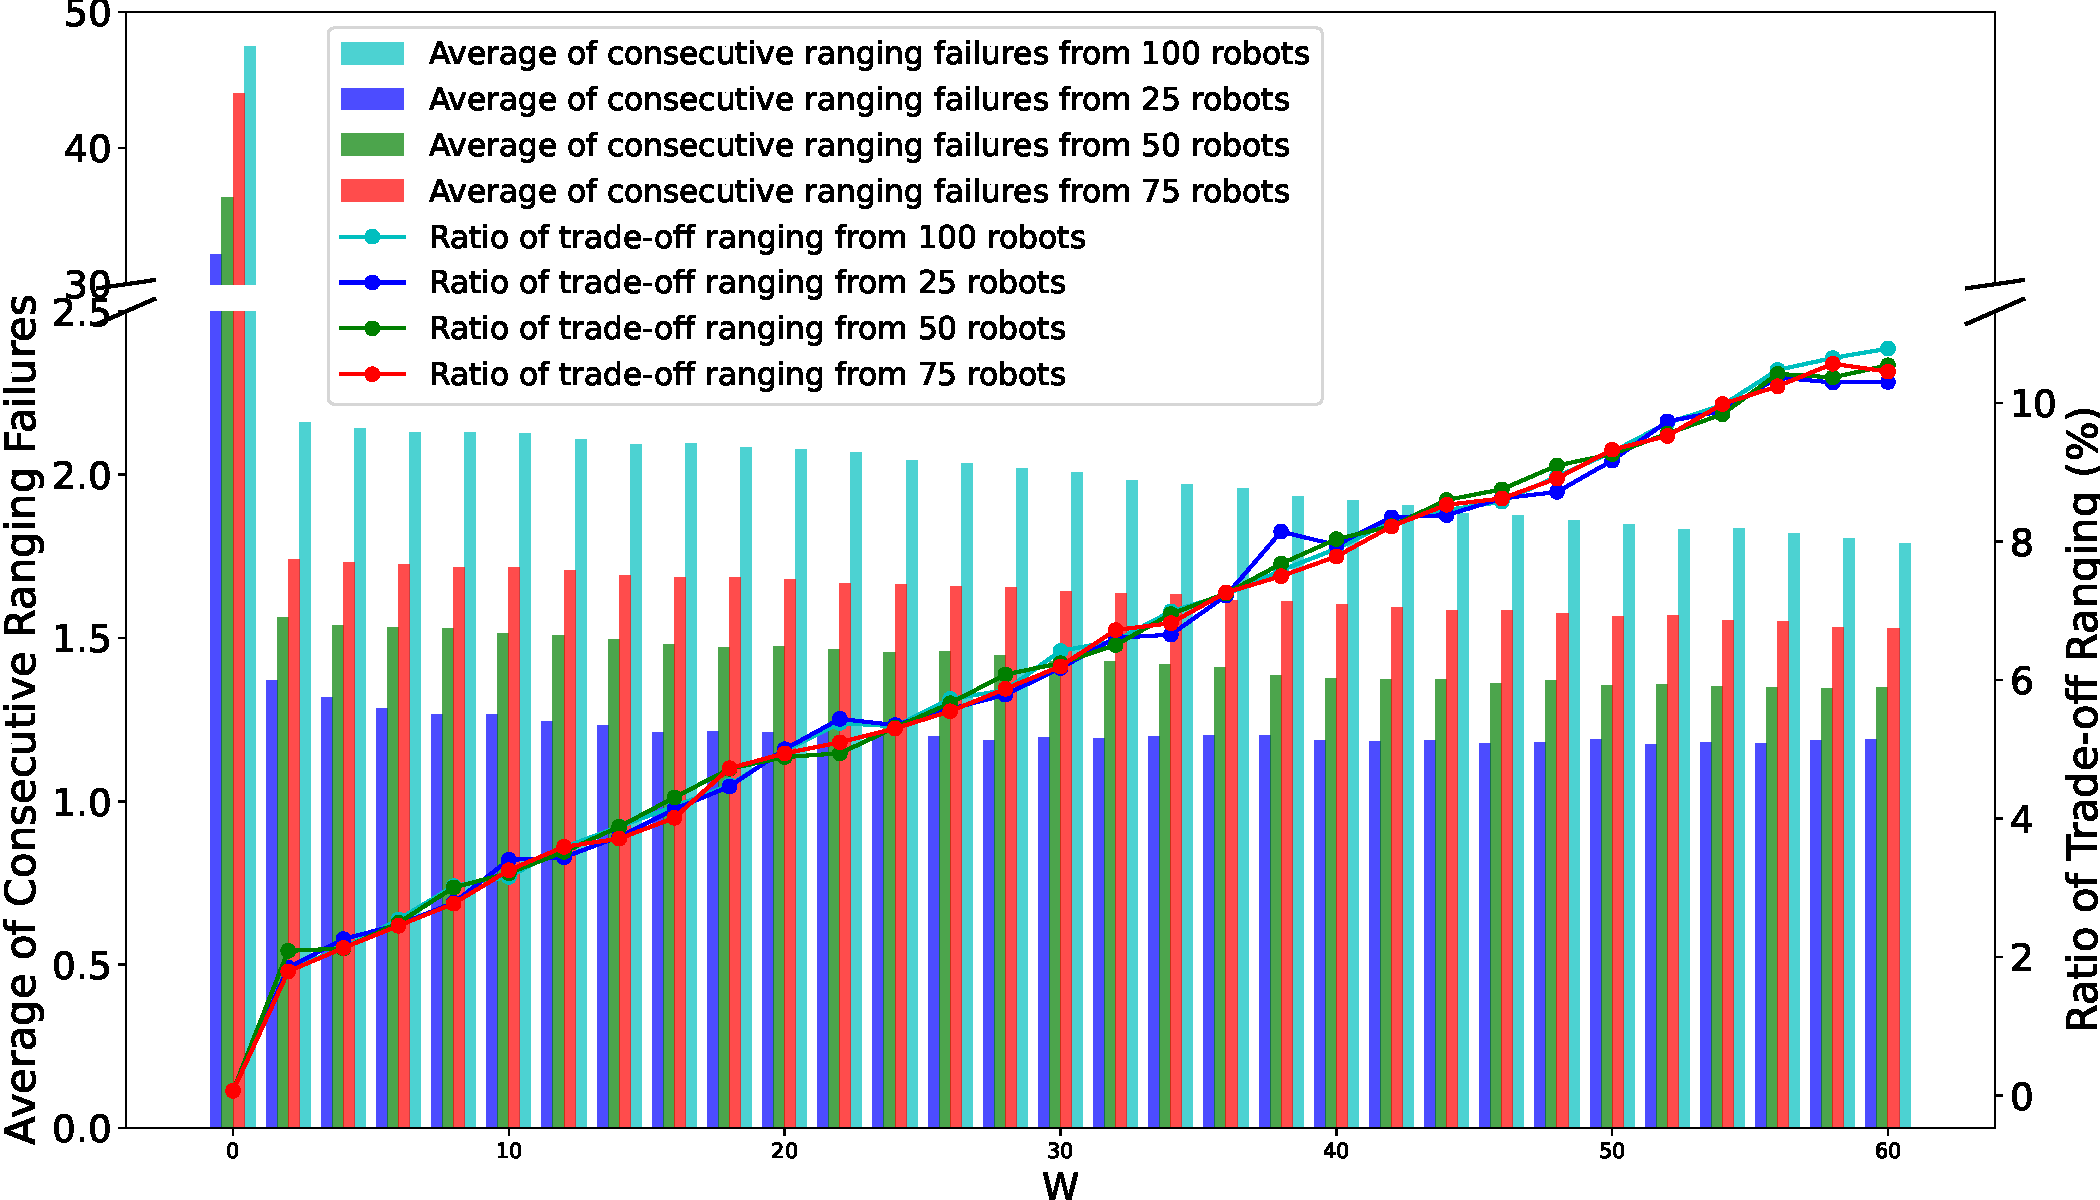
\includegraphics[width=0.8\textwidth]{figures/content/chapter3/robotsSimulation.pdf}}
\caption{
不同规模无人机集群在平均测距周期为100 ms、仿真时长为200s条件下的仿真结果
}
\label{fig:3_14}
\end{figure}
\subsection{真实世界中的鲁棒集群测距协议性能}
在本小节中，通过开展一系列大量真实世界中的无人机实验，对所提出测距协议的鲁棒性与准确性进行验证。

首先，在两台无人机执行测距的过程中，统计连续测距失败次数的平均值以及权衡测距的发生次数。
连续测距失败次数通过分析上一条成功接收报文的序列号进行计算；
权衡测距的概率则通过权衡测距发生次数与总测距次数之比进行统计。
在实验中，平均测距周期设置为 20 ms。
我们针对每一种不同的周期抖动取值，分别进行了 3 组实验，每组实验的测距持续时间为 120 s。
最终利用这些实验数据对相应的实验曲线进行拟合。

\begin{figure}[htbp]
  \centering
  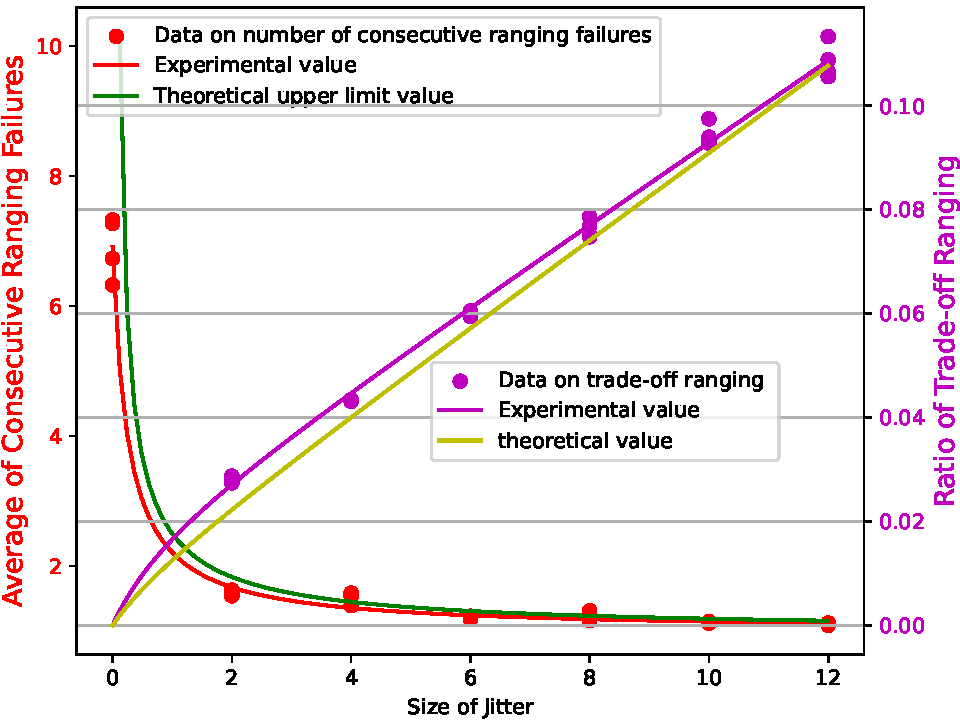
\includegraphics[width=.6\linewidth]{figures/content/chapter3/Comparison_TheoryandExperiment.pdf}
  \caption{鲁棒集群测距协议的理论分析与实验结果对比}
  \label{fig:3_15}
\end{figure}

如图\ref{fig:3_15}所示，实验结果与理论分析结果具有较高的一致性。
引入随机化周期后，连续测距失败的发生次数显著降低。
随着抖动幅度的增加，连续测距失败次数不再明显下降，而权衡测距发生的概率则持续快速上升。
真实实验结果验证了第\ref{sec:Theory}节中关于周期抖动对连续测距失败以及权衡测距概率影响的理论分析结论的正确性。

随后，我们在大规模无人机集群场景下对所提出的鲁棒集群测距协议的鲁棒性进行了系统评估。
通过逐步增大周期的抖动，观察连续测距失败次数的平均值、最大连续测距失败次数、权衡测距比例以及丢包率等指标的变化情况。
在实验设置中，共有 24 架无人机同时进行通信与测距，平均测距周期设置为 60 ms。
在 鲁棒集群测距协议运行过程中，对 120 s 内的数据进行了统计与分析。

\begin{figure}[htbp]
  \centering
  \includegraphics[width=.6\linewidth]{figures/content/chapter3/24RobotExpone.pdf}
  \caption{24 架无人机连续测距失败次数最大值与平均值的统计结果 }
  \label{fig:3_16}
\end{figure}

如图\ref{fig:3_16}所示，随着抖动幅度的增加，连续测距失败的平均值和最大值均呈现明显下降趋势。
在引入随机化周期后，这两个指标均出现显著降低，并且随着抖动值的进一步增大，其波动范围逐渐减小。
当抖动值大于 10 时，连续测距失败的最大值与平均值基本趋于稳定，不再发生明显变化。

\begin{table}[htbp]
\centering
\caption{24 架无人机实验中权衡测距比例与收包成功率统计结果}
\label{tab:jitter_results}

\resizebox{\textwidth}{!}{
\begin{tabular}{c|cccccccccc}
\hline
Jitter size & 0 & 2 & 4 & 6 & 8 & 10 & 14 & 20 & 30 & 40 \\
\hline
权衡测距比例
& 0.5\% & 0.7\% & 1.28\% & 1.86\% & 2.31\% & 3.58\% & 4.27\% & 6.34\% & 9.48\% & 12.3\% \\

收包成功率
& 85.49\% & 85.06\% & 85.13\% & 85.11\% & 85.04\% & 84.92\% & 85.24\% & 85.15\% & 84.96\% & 85.01\% \\
\hline
\end{tabular}
}

\end{table}

如表\ref{tab:jitter_results}所示，与第\ref{sec:Theory}节中的理论分析结果一致，权衡测距的比例随着抖动值的增大而逐渐上升。
同时，尽管测距周期引入了随机化，无人机集群的丢包率基本保持不变。
上述实验结果不仅验证了所提出协议在测距过程中能够有效缓解连续测距失败的问题，同时也为后续大规模实验中随机化周期参数的选择提供了重要参考。

\begin{figure}[htbp]
  \centering
  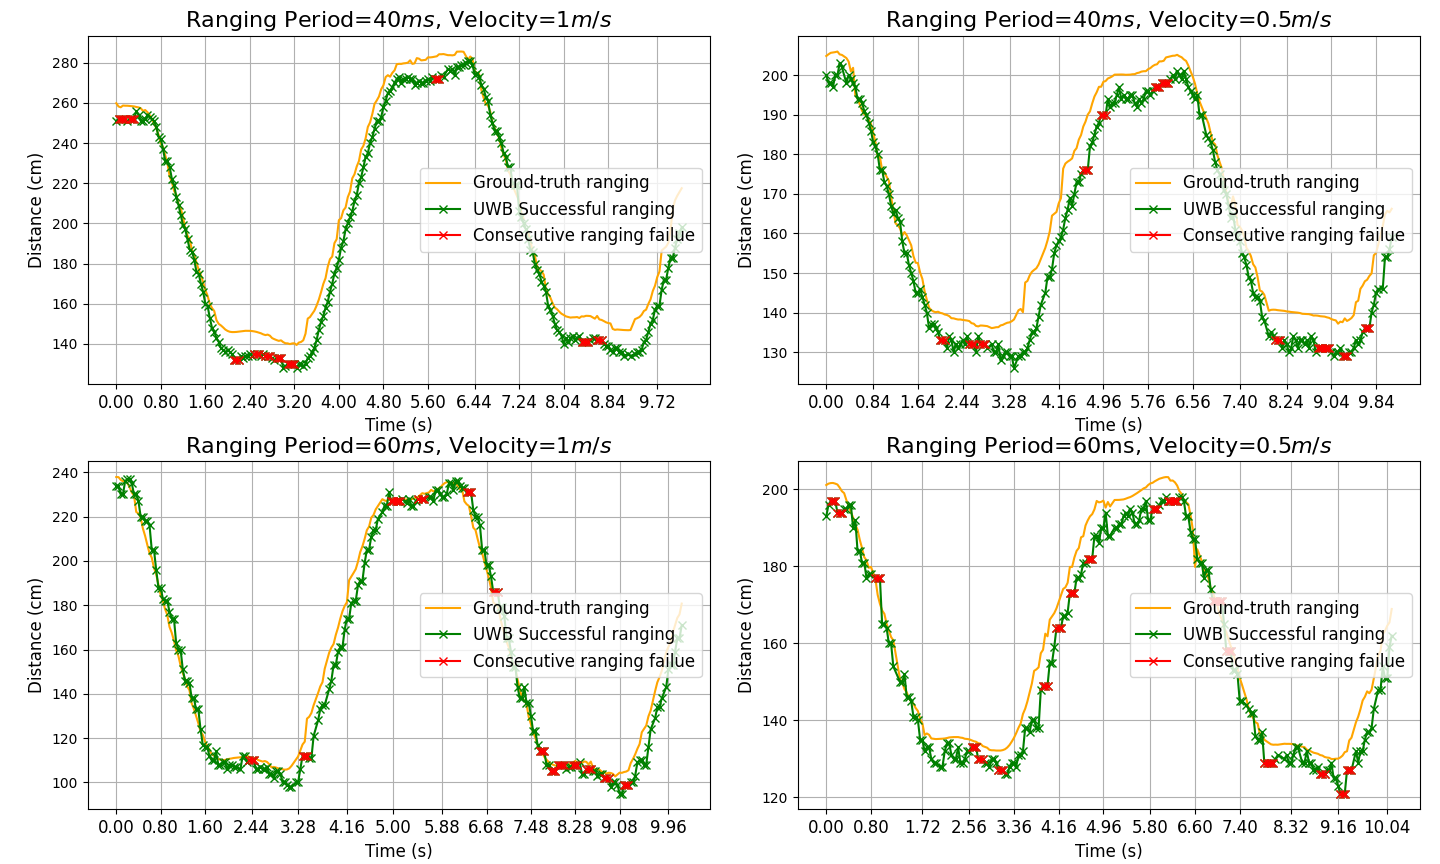
\includegraphics[width=.9\linewidth]{figures/content/chapter3/multiMeasurementsV2.png}
  \caption{应用鲁棒集群测距协议后，不同测距周期与速度下连续测距失败的缓解情况}
  \label{fig:3_17}
\end{figure}

最后，我们在图\ref{fig:3_16}所示的实验平台基础上，采用优化后的抖动参数设置的基础上，并在不同的运动速度和测距周期条件下进行了进一步实验。
实验结果如图\ref{fig:3_17}表明，在应用鲁棒集群测距协议后，与理论分析结果一致，测距失败在时间上呈现更加分散的分布特性，长时间连续测距失败现象不再出现。


\subsection{自适应协同定位算法性能}

为了评估所提出自适应协同定位算法的定位精度与稳定性，本文首先通过仿真实验对算法性能进行验证，并与传统扩展卡尔曼滤波方法进行对比分析。
实验主要关注在噪声统计特性未知或存在建模误差的情况下，算法对系统状态的估计能力。

在仿真中，系统采样周期设定为$\Delta t=0.1s$，每次实验包含 100 个时间步。为了保证实验结果的统计稳定性，每组实验进行 100 次 蒙特卡洛重复仿真，并对结果取平均值。
实验中一无人机静止，另一无人机以1 m/s 的速度匀速向前运动，其中过程噪声协方差矩阵$\Omega_{0} = =\operatorname{diag}(0.2^2,0.2^2,0.3^2,0.2^2,0.2^2, 0.3^2)$, 
量测噪声为高斯白噪声，其协方差设定为 $\Lambda_{0} = 0.1^2$​。
初始协方差矩阵设定为 $\Sigma_{ij,0} = =\operatorname{diag}(5,5,0.1)$

为了评估所提出算法的性能，本文选取以下两种方法进行对比：第一种传统扩展卡尔曼滤波
采用标准扩展卡尔曼滤波进行状态估计，量测噪声协方差在整个滤波过程中保持固定。
第二种为本文提出的自适应扩展卡尔曼滤波，在每个时刻通过迭代更新状态估计、协方差矩阵以及量测噪声协方差，实现对系统不确定性的自适应估计。
为了研究迭代次数对算法性能的影响，本文分别设置迭代次数 $N=1,2,3,4,5$。

本文采用位置均方根误差（Root Mean Square Error，RMSE）作为算法性能评价指标：
\begin{equation}
R M S E=\sqrt{\frac{1}{T} \sum_{k=1}^{T}\left\|\hat{p}_{k}-p_{k}\right\|^{2}}
\end{equation}
其中：$p_{k}$  为真实位置,$\hat{p}_{k}$  为估计位置, $T$  为仿真步数.

\begin{figure}[htbp]
  \centering
  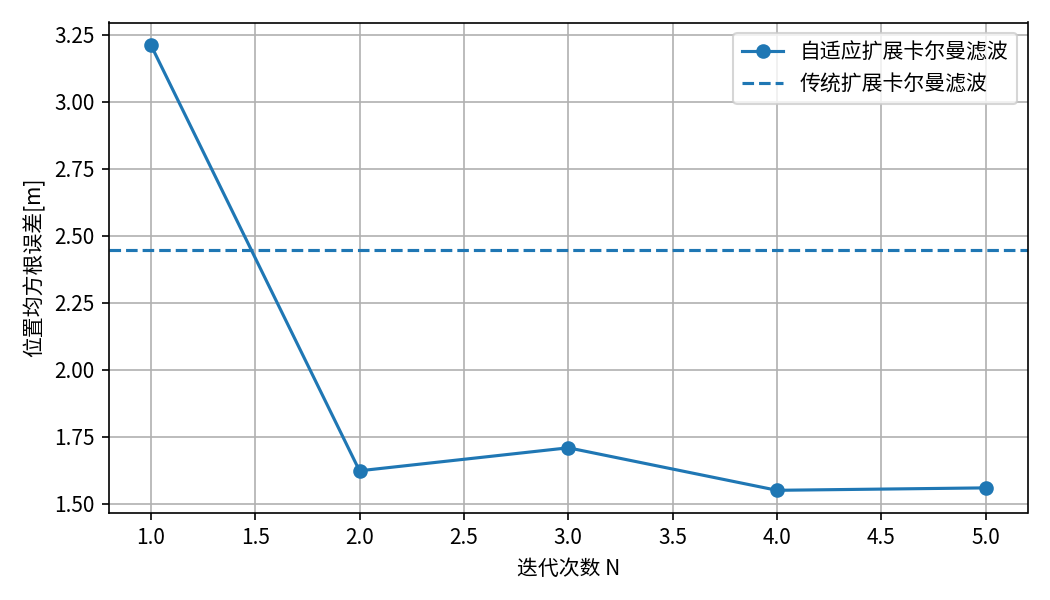
\includegraphics[width=.7\linewidth]{figures/content/chapter3/AEKF.png}
  \caption{自适应EKF与传统EKF定位误差对比图}
  \label{fig:3_19}
\end{figure}

从实验结果图\ref{fig:3_19}中可以看出，不同迭代次数下算法的定位误差均方根变化情况，并与传统扩展卡尔曼滤波的定位误差进行了对比。
图中横轴表示迭代次数 N，纵轴表示位置估计误差的均方根值，虚线表示传统 EKF 算法的定位误差水平。

当迭代次数 N = 1 时，算法的 RMSE 约为 3.2 m，此时误差较大，说明在未进行充分迭代优化的情况下，状态估计精度仍然较低。
随着迭代次数增加，定位误差明显下降。当 N = 2 时，RMSE 降至约 1.62 m，相较于传统 EKF 的约 2.45 m，定位精度得到明显提升。
当迭代次数继续增加时，RMSE 的变化逐渐趋于稳定。
结果表明，当迭代次数达到 4 次左右时，算法的估计精度已经基本收敛，继续增加迭代次数对精度提升的作用较为有限。

与传统 EKF 算法相比，所提出的迭代算法在 N ≥ 2 时均表现出更低的定位误差，RMSE 从 EKF 的约 2.45 m 降低到约 1.55 m，误差降低约 36\%。

综上所述，仿真结果验证了所提出算法在定位精度方面相较于传统 EKF 具有明显优势，并且在迭代次数达到一定程度后能够快速收敛，在保证定位精度的同时兼顾计算效率。

\begin{figure}[htbp]
  \centering
  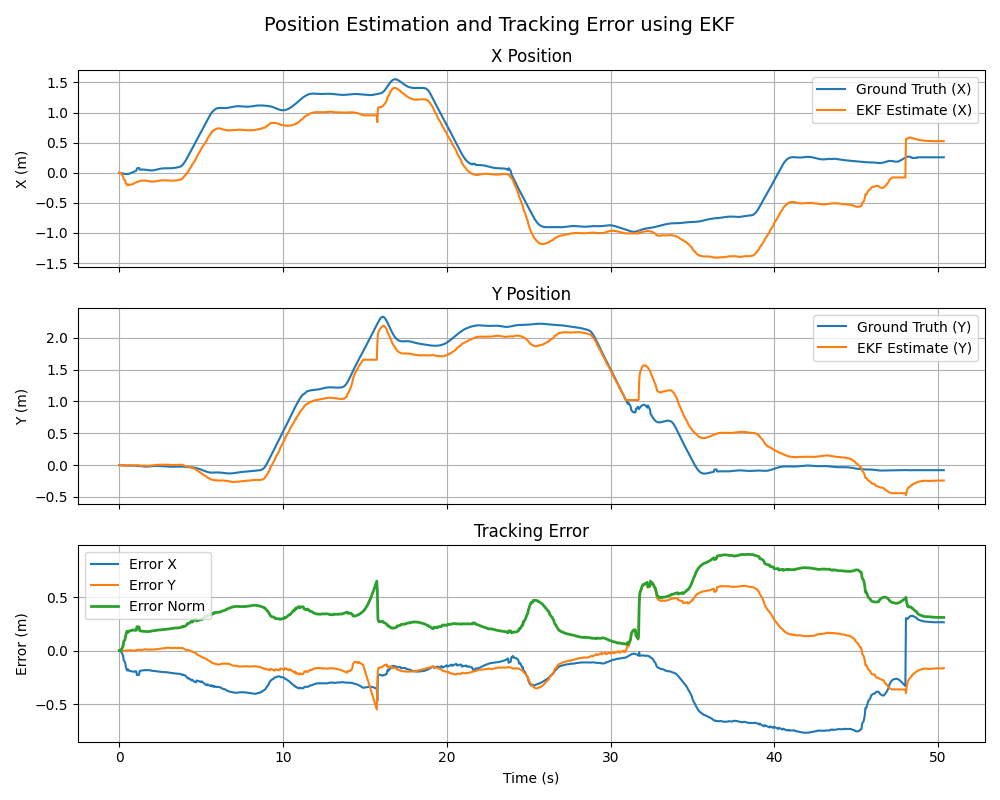
\includegraphics[width=.6\linewidth]{figures/content/chapter3/EKFError.png}
  \caption{传统EKF定位误差图}
  \label{fig:3_20}
\end{figure}
为验证所提出自适应扩展卡尔曼滤波算法在无人机相对定位中的性能，本文设计并开展了双无人机相对定位实验。
在实验场景中，选取两架无人机，其中一架无人机保持悬停状态，作为参考节点；
另一架无人机执行预设轨迹飞行，其运动轨迹为边长为 1m×1m 的正方形路径。
该实验设计能够构建具有代表性的动态相对运动场景，有利于评估定位算法在实际飞行过程中的跟踪性能与稳定性。

在测量方面，系统采用超宽带模块进行相对距离观测，测距平均周期约为60 ms。基于前文的鲁棒集群测距协议，在测距周期中引入幅值为6ms的随机扰动，使得测距的结果更为鲁棒。
同时，在滤波过程中，AEKF算法基于上述仿真实验的分析在每一时刻执行3次迭代更新，以增强对非线性系统的逼近能力，提高状态估计精度。

实验过程中，通过Vicon光学运动捕捉系统获取高精度位置数据，作为真实值（Ground Truth）。
将滤波器输出的估计位置与真实值进行对比，从而计算定位误差并评估算法性能。


\begin{table}[htbp]
\centering
\caption{两种算法定位误差统计对比}
\label{tab:error_comparison}
\begin{tabular}{lccc}
\toprule
算法类型 & X 轴 (m) & Y 轴 (m) & 总误差 (m) \\
\midrule
传统 EKF & 0.3896 & 0.2715 & 0.4749 \\
自适应 AEKF & \textbf{0.1651} & \textbf{0.1868} & \textbf{0.2493} \\
\bottomrule
\end{tabular}
\end{table}



实验分别运行基于传统扩展卡尔曼滤波（EKF）和自适应扩展卡尔曼滤波（AEKF）的定位计算，记录目标无人机在 $X$ 轴与 $Y$ 轴方向的实时位置误差。
具体的误差统计数据如表\ref{tab:error_comparison}所示。



AEKF 算法的总均方根误差（RMSE）为 0.2493 m，相较于传统 EKF 算法的 0.4749 m，定位精度提升了约 47.5\%。
\begin{figure}[htbp]
  \centering
  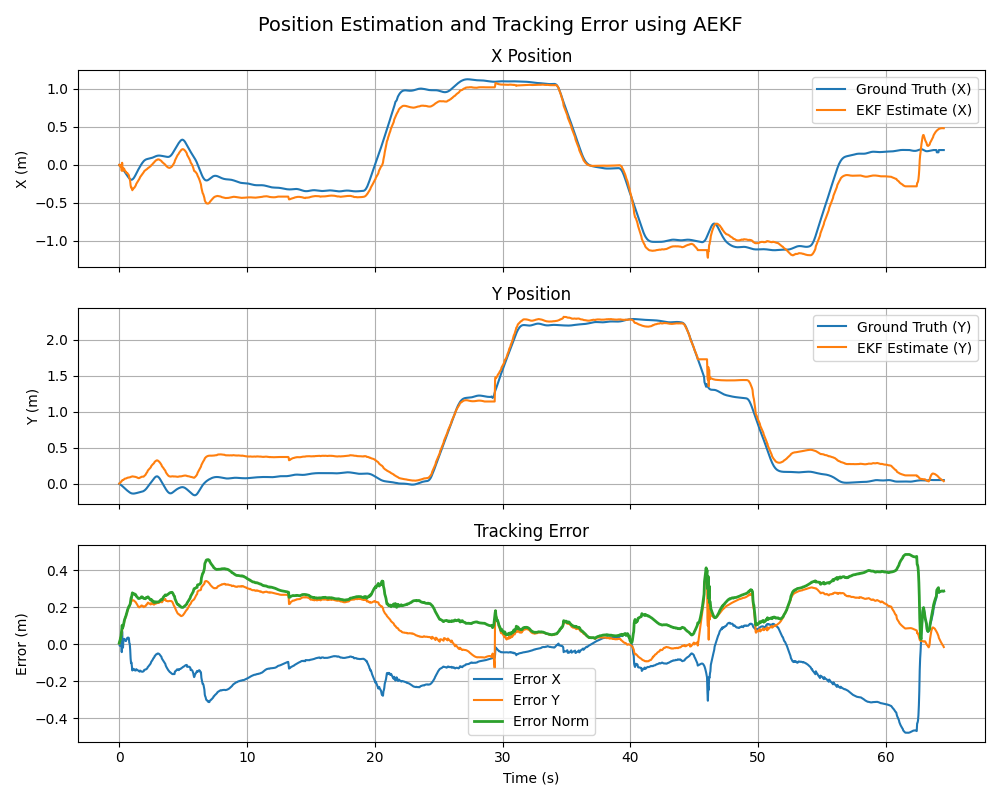
\includegraphics[width=.6\linewidth]{figures/content/chapter3/AEKFError.png}
  \caption{自适应EKF定位误差图}
  \label{fig:3_21}
\end{figure}
图 \ref{fig:3_20} 与图 \ref{fig:3_21} 分别展示了传统扩展卡尔曼滤波（EKF）与自适应扩展卡尔曼滤波（AEKF）在双机协同定位实验中的位置估计与跟踪误差时域曲线。
各子图中，蓝色曲线表示地面真实轨迹，橙色曲线表示滤波估计轨迹；
底部误差子图中，蓝色、橙色与绿色曲线分别对应 X 轴误差、Y 轴误差及总误差范。

对比两图的上部位置跟踪曲线可以观察到：传统 EKF：在目标无人机执行 1 m × 1 m 正方形轨迹的转弯机动阶段（约 $t = 2.5$ s、$5.0$ s、$7.5$ s 等时刻），估计轨迹与真实轨迹之间存在肉眼可辨的滞后与超调现象。尤其在 Y 轴方向，当无人机由上升段转入平飞段时，EKF 估计值未能及时响应运动状态的变化，导致橙色曲线明显偏离蓝色真实值。
自适应 AEKF：在全飞行时段内，橙色估计曲线与蓝色真实曲线几乎紧密贴合。即便在正方形四个顶点的急转弯处，AEKF 仍能保持对真实轨迹的高保真跟踪，未见明显的滞后或过冲。这表明自适应协方差调整机制能够实时感知机动状态的变化，并动态增强滤波器对观测新息的响应能力。

上述实验结果表明，所采用的自适应 EKF 算法在仅增加少量计算迭代次数的前提下，能够有效克服传统 EKF 在动态环境及测距抖动下的精度发散问题。
该算法在保证厘米级定位精度的同时，为后续的大规模集群编队飞行提供了可靠的相对定位数据支撑。
\subsection{  大型集群编队飞行实验}

本小节展示了一项真实飞行实验，用于验证领导-跟随编队控制的效果。
实验中基于上文的自适应协同定位算法实现无人机之间的相对定位。
实验共使用13架Crazyflie无人机，初始时各无人机间距为1米。
在飞行过程中，9架无人机在边长为2 m的内环区域飞行，其余4架无人机在边长为4 m的外环区域飞行。
平均测距周期为60 ms，抖动设置为6。
飞行过程如图\ref{fig:3_22}所示，四张图分别展示了无人机的初始位置、跟随阶段以及编队变化阶段。
红色圆圈表示领航无人机，其他颜色圆圈表示跟随无人机。

\begin{figure}[htbp]
  \centering
  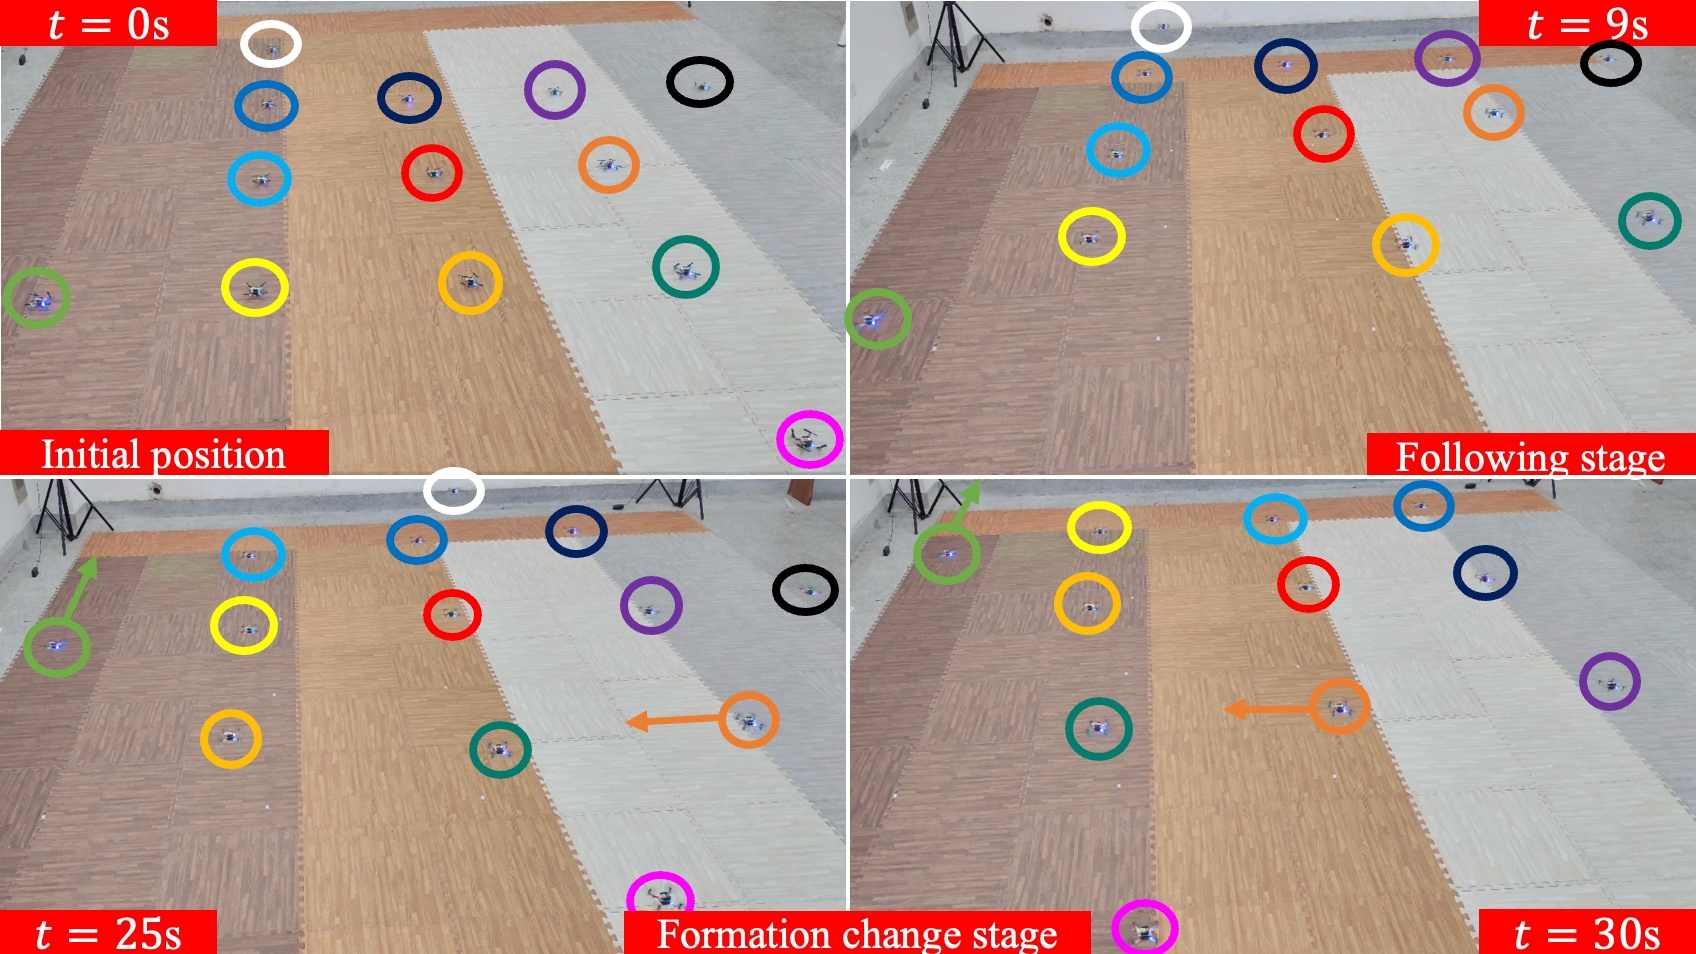
\includegraphics[width=.7\linewidth]{figures/content/chapter3/uwb_13_formation.png}
  \caption{13架无人机编队飞行的顶部视图}
  \label{fig:3_22}
\end{figure}

在 t= 0 s时，所有无人机从各自已知的初始位置起飞；
经过5秒后，无人机已形成编队，并保持与红色圆圈编号为1的无人机的相对位置，该无人机以随机方式飞行。
从 t= 15 s开始，所有无人机开始改变编队，图中箭头表示下一步编队变化的方向。
此外，在编队飞行过程中，记录了4架无人机相对于橙色圆圈（编号为2的无人机）的UWB测距数据及地面真实距离，如图\ref{fig:3_23}(a)所示。
图\ref{fig:3_23}显示了测距误差分布，两架无人机之间距离测量的平均绝对误差约为6.21 cm。

\begin{figure}[ht]
    \centering
    
    \begin{minipage}[b]{0.5\textwidth}
        \centering
        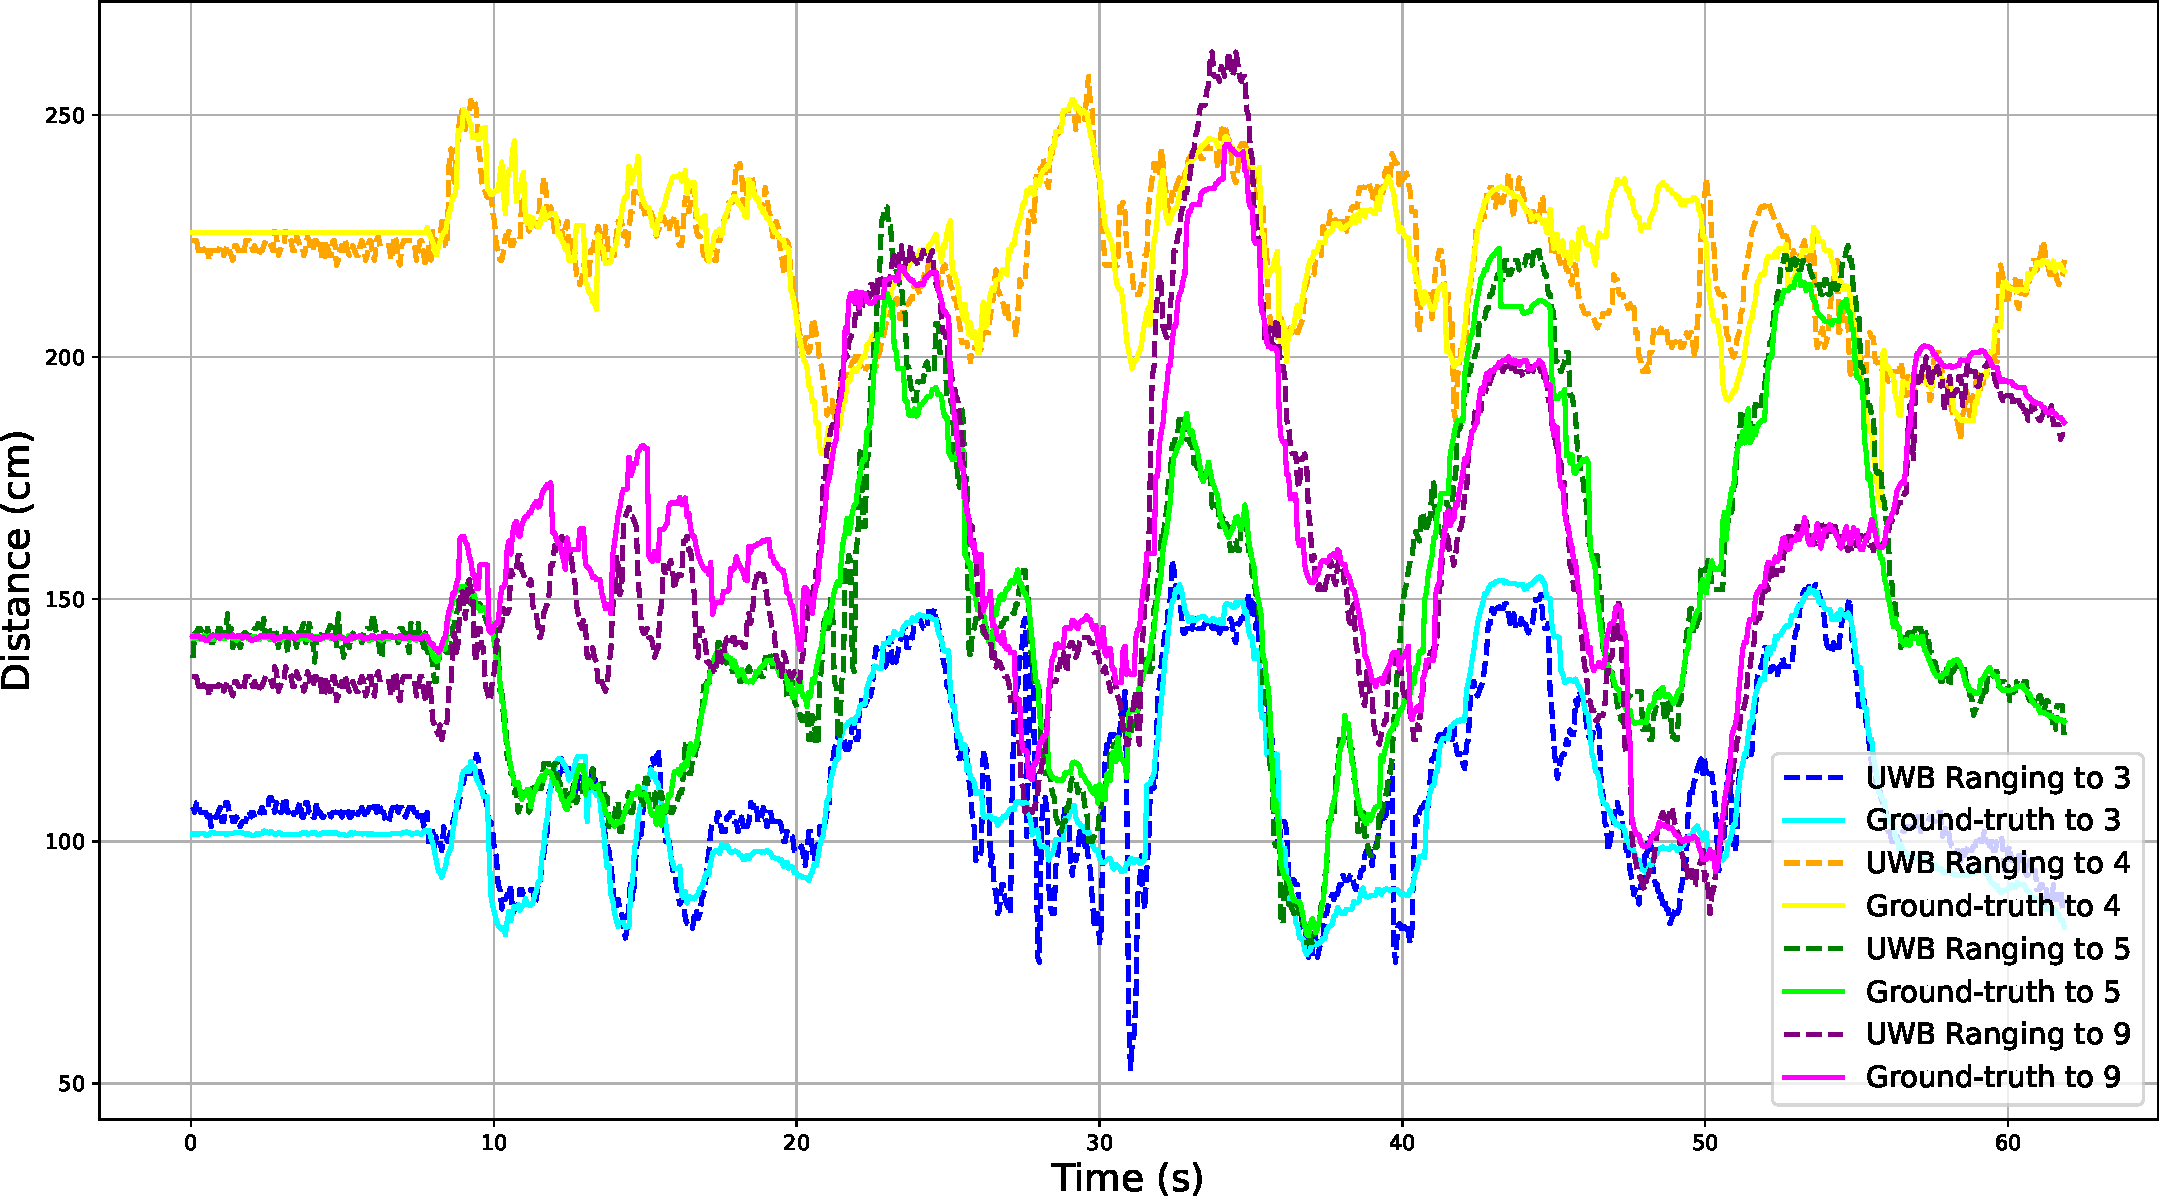
\includegraphics[width=\textwidth, trim={0cm 0cm 0cm 0cm}, clip]{figures/content/chapter3/uwb_4_distance.pdf}
        \\(a) UWB测距结果
    \end{minipage}
    \begin{minipage}[b]{0.3\textwidth}
        \centering
        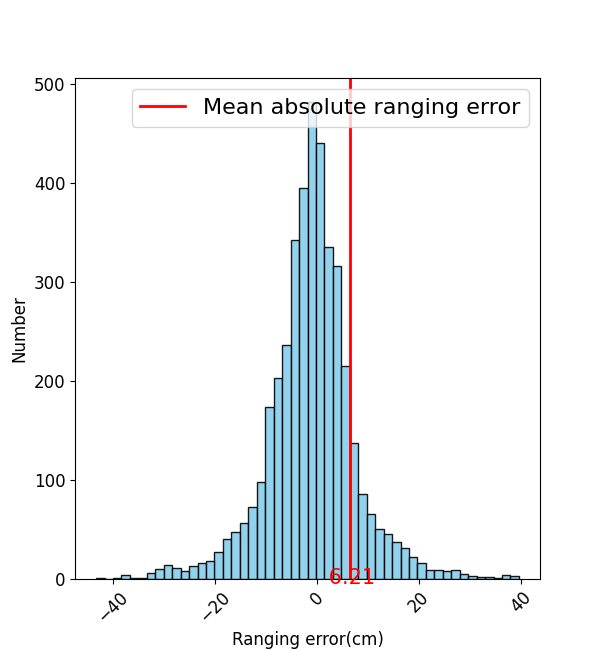
\includegraphics[width=\textwidth, trim={0.2cm 0cm 0cm 0.3cm}, clip]{figures/content/chapter3/errorDistribution.png}
        \\(b) 测距误差分布
    \end{minipage}
    \caption{13架无人机编队飞行过程中获取的5架无人机测量数据}
    \label{fig:3_23}
\end{figure}

实验结果表明，所提出的无人机集群自适应协同定位算法在动态且密集的大规模无人机群中，能够实现稳健且精确的距离测量。
因此，该算法可为大规模无人机群的高效定位和自主编队飞行任务提供可靠支持。

\section{本章小节}

本章针对无人机集群相对定位问题，提出了一种基于 UWB 的自适应协同定位方法。
首先，为解决大规模集群中测距冲突和连续测距失败的问题，设计了一种鲁棒集群测距协议，并通过引入周期抖动机制以及权衡测距方法，提高了测距成功率和系统稳定性。
随后，在扩展卡尔曼滤波框架下引入期望最大化算法，实现对系统噪声参数的在线估计，从而提升无人机协同定位的精度与鲁棒性。
通过仿真实验和真实无人机编队飞行实验对所提出方法进行了验证，实验结果表明该方法能够在多无人机动态环境中实现稳定且高精度的相对定位。

